% Presentación para la defensa del proyecto final.
% Estructura según ../PLAN_DEFENSA.md. Reusa imágenes y diagramas del informe.
% Compilar (desde informe/presentacion): tectonic -X compile presentacion.tex, o guardar en VS Code
\documentclass[aspectratio=169,10pt]{beamer}

\usepackage[spanish,es-noshorthands,es-nodecimaldot]{babel}
\usepackage{fontspec}
\usepackage{amsmath,amssymb}
\usepackage{booktabs}
\usepackage{siunitx}
\sisetup{output-decimal-marker={,}, per-mode=symbol}
\usepackage{tikz}
\usetikzlibrary{positioning, arrows.meta, shapes.geometric, fit, calc}
\usepackage{listings}

\graphicspath{{../Imagenes/}}

%%%%%%%% ESTILO %%%%%%%%
\usetheme{default}
\definecolor{unsazul}{RGB}{0,51,102}
\definecolor{acento}{RGB}{214,104,0}
\setbeamercolor{frametitle}{fg=white,bg=unsazul}
\setbeamercolor{title}{fg=unsazul}
\setbeamercolor{structure}{fg=unsazul}
\setbeamercolor{alerted text}{fg=acento}
\setbeamerfont{frametitle}{series=\bfseries}
\setbeamertemplate{navigation symbols}{}
\setbeamertemplate{itemize items}[circle]
\setbeamertemplate{frametitle}{%
  \nointerlineskip
  \begin{beamercolorbox}[wd=\paperwidth,ht=2.4ex,dp=1.2ex,leftskip=1em]{frametitle}
    \usebeamerfont{frametitle}\insertframetitle
  \end{beamercolorbox}}
\setbeamertemplate{footline}{%
  \hfill\textcolor{gray}{\scriptsize Telerobótica -- UNS DIEC \quad \insertframenumber}\hspace{1em}\vspace{0.8ex}}

% Lo que falta completar (en rojo, como en el informe)
\newcommand{\pendiente}[1]{\textcolor{red}{\textbf{[PENDIENTE:} #1\textbf{]}}}

\tikzset{
  bloque/.style={draw, rounded corners, align=center, fill=blue!5, minimum height=1cm, font=\small},
  flecha/.style={-{Stealth[length=2.5mm]}, thick},
}

\lstset{language=C++, basicstyle=\ttfamily\scriptsize, keywordstyle=\color{blue},
  commentstyle=\color{green!50!black}, backgroundcolor=\color{gray!8}, frame=single,
  rulecolor=\color{gray!40}, showstringspaces=false, columns=fullflexible,
  morekeywords={uint8_t,uint16_t,int16_t}}

\title{Movilidad de mano impresa en 3D\\en base al sensado de los movimientos}
\subtitle{Telerobótica -- Proyecto Final}
\author{Joaquín Petruf \and Sebastián Amoroso}
\institute{Tutores: Rodrigo Martín Santos, Gabriel Eggly\\[0.5ex]
  Ingeniería Electrónica -- DIEC -- Universidad Nacional del Sur}
\date{\pendiente{fecha de la defensa}}

\begin{document}

%%%%%%%%%%%%%%%%%%%%%%%%%%%%%%%%%%%%%%%%%%%%%%%%%%%%%%%%%%%%%%%%%%%
\begin{frame}[plain]
  \begin{columns}[T]
    \column{0.5\textwidth}
\includegraphics[height=1.6cm]{EmblemaUNS.jpg}
    \column{0.5\textwidth}\hfill
\includegraphics[height=1.6cm]{DIEC.jpg}
  \end{columns}
  \vfill
  \titlepage
\end{frame}

%%%%%%%%%%%%%%%%%%%%%%%%%%%%%%%%%%%%%%%%%%%%%%%%%%%%%%%%%%%%%%%%%%%
\begin{frame}{Motivación}
  \begin{columns}[c]
    \column{0.58\textwidth}
    \begin{itemize}
      \item Tareas donde la presencia humana es un \alert{riesgo inaceptable}:
      \begin{itemize}
        \item sustancias tóxicas y reactivos volátiles
        \item material radiactivo
        \item temperaturas extremas
      \end{itemize}
      \item \textbf{Telerobótica:} un operador maneja un robot a distancia, a través de un enlace (en general inalámbrico).
      \item Interfaz natural: la propia mano del operador.
    \end{itemize}
    \column{0.42\textwidth}
    \begin{block}{Idea}
      Sensar los movimientos de una mano humana y \textbf{replicarlos de forma inalámbrica} en una mano impresa en 3D.
    \end{block}
  \end{columns}
\end{frame}

%%%%%%%%%%%%%%%%%%%%%%%%%%%%%%%%%%%%%%%%%%%%%%%%%%%%%%%%%%%%%%%%%%%
\begin{frame}{Objetivo y componentes}
  \textbf{Movimientos que se replican:}
  \begin{itemize}
    \item Apertura y cierre de los \textbf{5 dedos}, en forma individual
    \item \textbf{Rotación} de la muñeca (pronosupinación)
    \item \textbf{Flexión y extensión} de la muñeca
  \end{itemize}
  \vspace{1ex}
  \begin{columns}[T]
    \column{0.45\textwidth}
    \centering\textbf{Guante (transmisor)}\\[1ex]
    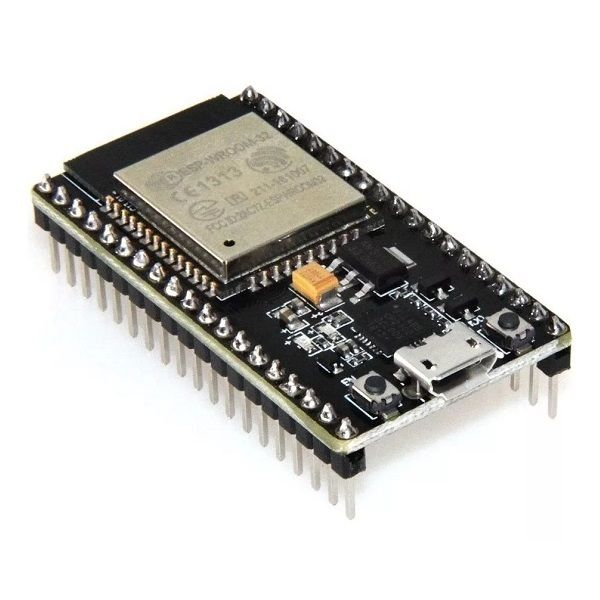
\includegraphics[height=1.9cm]{ESP32.jpeg}\hspace{1mm}
    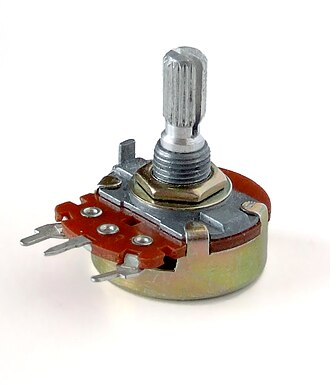
\includegraphics[height=1.9cm]{Potenciometro.jpg}\hspace{1mm}
    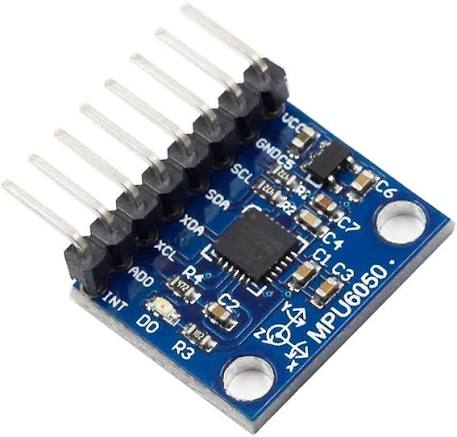
\includegraphics[height=1.9cm]{MPU6050.jpg}\\
    {\scriptsize ESP32 \quad 5 potenciómetros \quad IMU MPU6050}
    \column{0.45\textwidth}
    \centering\textbf{Mano robótica (receptor)}\\[1ex]
    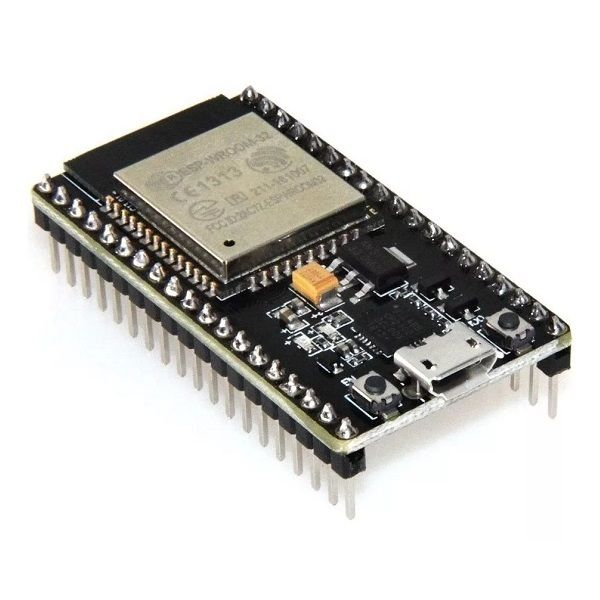
\includegraphics[height=1.9cm]{ESP32.jpeg}\hspace{1mm}
    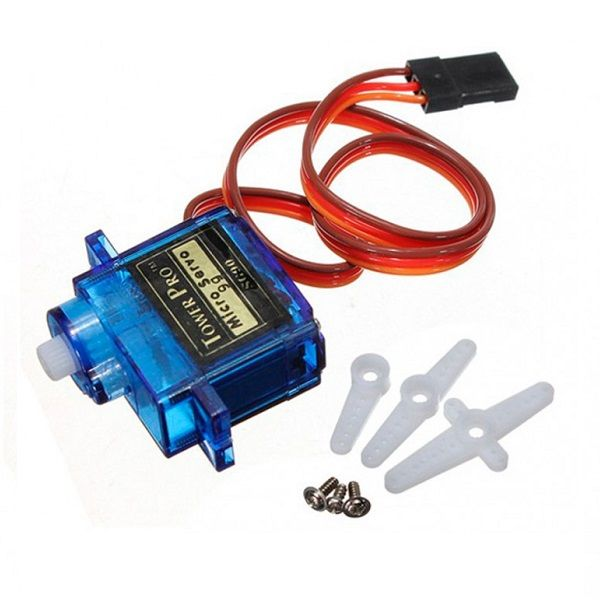
\includegraphics[height=1.9cm]{SG90.jpeg}\hspace{1mm}
    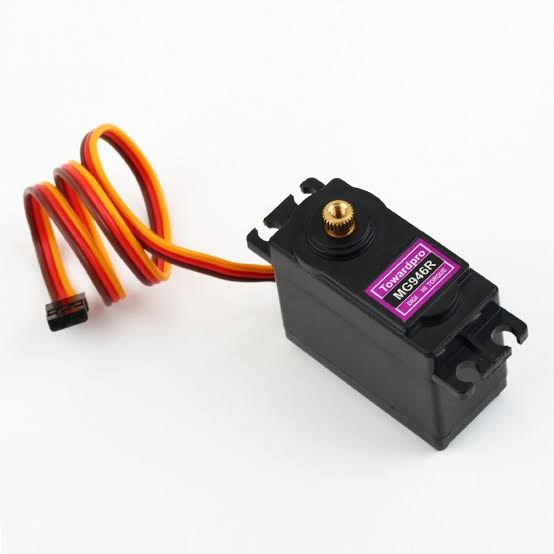
\includegraphics[height=1.9cm]{MG946R.jpg}\\
    {\scriptsize ESP32 \quad 5 $\times$ SG90 (dedos) \quad 2 $\times$ MG946R (muñeca)}
  \end{columns}
\end{frame}

%%%%%%%%%%%%%%%%%%%%%%%%%%%%%%%%%%%%%%%%%%%%%%%%%%%%%%%%%%%%%%%%%%%
\begin{frame}{Demostración}
  \centering
  \begin{tikzpicture}
    \node[draw=unsazul, very thick, rounded corners, minimum width=11cm, minimum height=5.2cm,
          fill=gray!10, align=center, font=\large] {%
      \textbf{Demo en vivo}\\[2ex]
      \normalsize Video de respaldo:\\
      \pendiente{grabar el video y enlazarlo aquí}};
  \end{tikzpicture}
  % Para enlazar el video (se abre con el reproductor del sistema):
  % \href{run:video/demo.mp4}{\includegraphics[width=11cm]{captura_demo.png}}
\end{frame}

%%%%%%%%%%%%%%%%%%%%%%%%%%%%%%%%%%%%%%%%%%%%%%%%%%%%%%%%%%%%%%%%%%%
\begin{frame}{Arquitectura del sistema}
  \centering
  \resizebox{\textwidth}{!}{%
  \begin{tikzpicture}[node distance=0.6cm and 1.2cm]
    \node[bloque] (pot) {5 potenciómetros\\(dedos)};
    \node[bloque, below=of pot] (imu) {MPU6050\\(muñeca)};
    \coordinate (medio) at ($(pot)!0.5!(imu)$);
    \node[bloque, right=1.9cm of medio, fill=orange!10, minimum width=3.4cm] (tx)
         {\textbf{ESP32 Transmisor}\\ ADC sobremuestreado\\ Filtro complementario\\ Ángulos de servo\\ Empaquetado + checksum};
    \node[draw, dashed, rounded corners, inner sep=6pt, fit=(pot)(imu)(tx), label=above:{\textbf{Guante}}] {};
    \node[bloque, right=1.7cm of tx, fill=green!10, minimum width=3.4cm] (rx)
         {\textbf{ESP32 Receptor}\\ Validación del paquete\\ Supervisión (failsafe)\\ Limitador de velocidad\\ Banda muerta};
    \node[bloque, right=of rx, yshift=0.8cm] (sg) {5 servos SG90\\(dedos)};
    \node[bloque, right=of rx, yshift=-0.8cm] (mg) {2 servos MG946R\\(muñeca)};
    \node[draw, dashed, rounded corners, inner sep=6pt, fit=(rx)(sg)(mg), label=above:{\textbf{Mano robótica}}] {};
    \draw[flecha] (pot) -- (tx);
    \draw[flecha] (imu) -- (tx);
    \draw[flecha, very thick, blue!60!black] (tx) -- node[above, font=\footnotesize, align=center]{ESP-NOW\\2,4 GHz} node[below, font=\footnotesize, align=center]{19 bytes\\50 Hz} (rx);
    \draw[flecha] (rx) -- node[above, font=\footnotesize]{PWM} (sg);
    \draw[flecha] (rx) -- node[below, font=\footnotesize]{PWM} (mg);
  \end{tikzpicture}}
  \vspace{2ex}
  \begin{alertblock}{Decisión de diseño}
    El guante \textbf{calcula todo} y envía ángulos de servo; la mano sólo \textbf{valida, suaviza y mueve}.
    Si cambia el operador, se recalibra el guante sin tocar la mano.
  \end{alertblock}
\end{frame}

%%%%%%%%%%%%%%%%%%%%%%%%%%%%%%%%%%%%%%%%%%%%%%%%%%%%%%%%%%%%%%%%%%%
\begin{frame}{Transmisor: el guante}
  \begin{columns}[c]
    \column{0.5\textwidth}
    \centering
    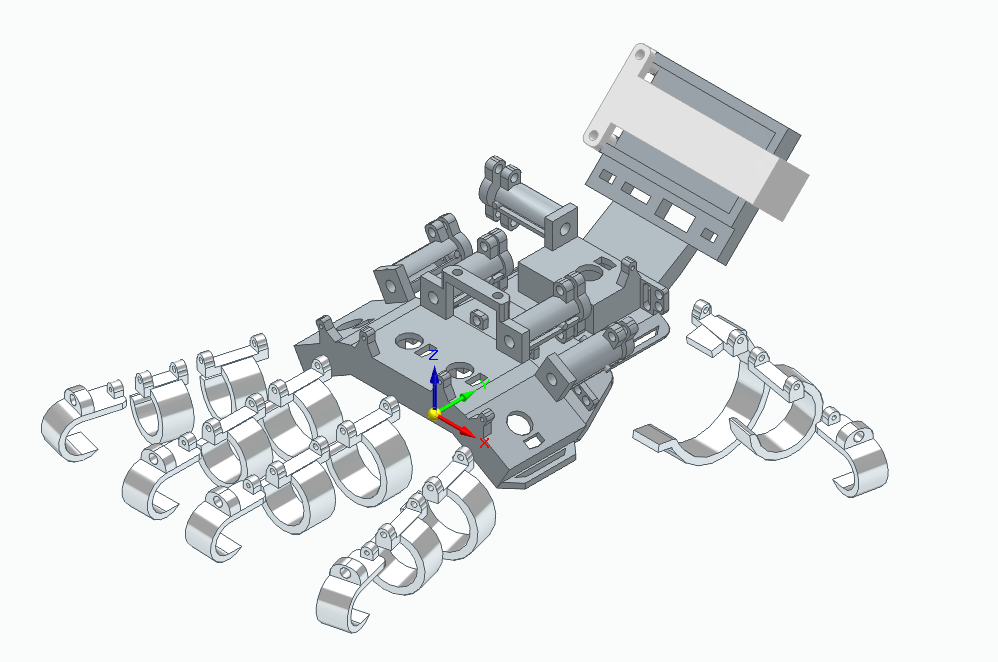
\includegraphics[width=\linewidth]{Transmisor/GuanteCompleto.png}\\
    {\scriptsize Diseño en Solid Edge, impreso en 3D}\\[1ex]
    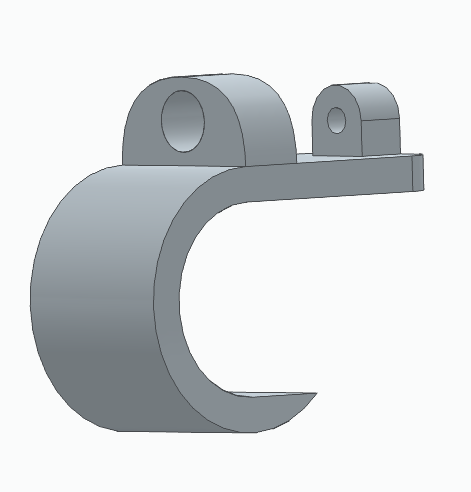
\includegraphics[height=1.5cm]{Transmisor/Dedal_1.png}\hspace{2mm}
    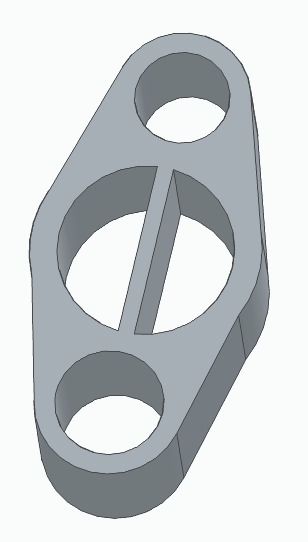
\includegraphics[height=1.5cm]{Transmisor/Palanca_Pote.jpg}\hspace{2mm}
    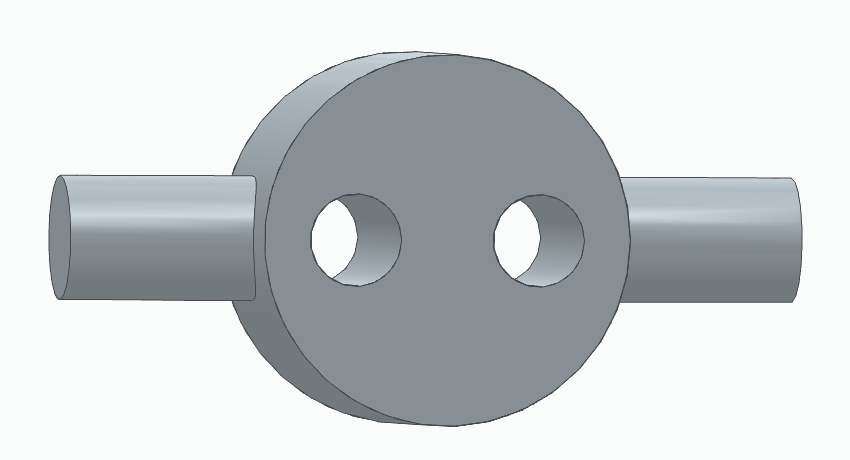
\includegraphics[height=1.5cm]{Transmisor/Resortera.png}\\
    {\scriptsize Dedal \quad Palanca del potenciómetro \quad Resortera}
    \column{0.5\textwidth}
    \textbf{Del dedo al potenciómetro:}
    \begin{enumerate}\small
      \item Una \textbf{tanza} atada al dedal de la punta recorre el dorso del dedo, guiada por dedales en cada falange
      \item En el dorso tira de una \textbf{palanca} montada en el eje del potenciómetro
      \item Sigue por un tubo con \textbf{resorte} hasta la resortera
      \item Al abrir el dedo, el resorte devuelve el eje al reposo y mantiene la tanza tensa (menos holgura)
    \end{enumerate}
    \vspace{1ex}
    \begin{itemize}\small
      \item MPU6050 paralelo al dorso de la mano
      \item ESP32 en la muñeca, alimentado por USB desde la PC (calibración y telemetría)
    \end{itemize}
  \end{columns}
\end{frame}

\begin{frame}{Transmisor: conexionado}
  \centering
  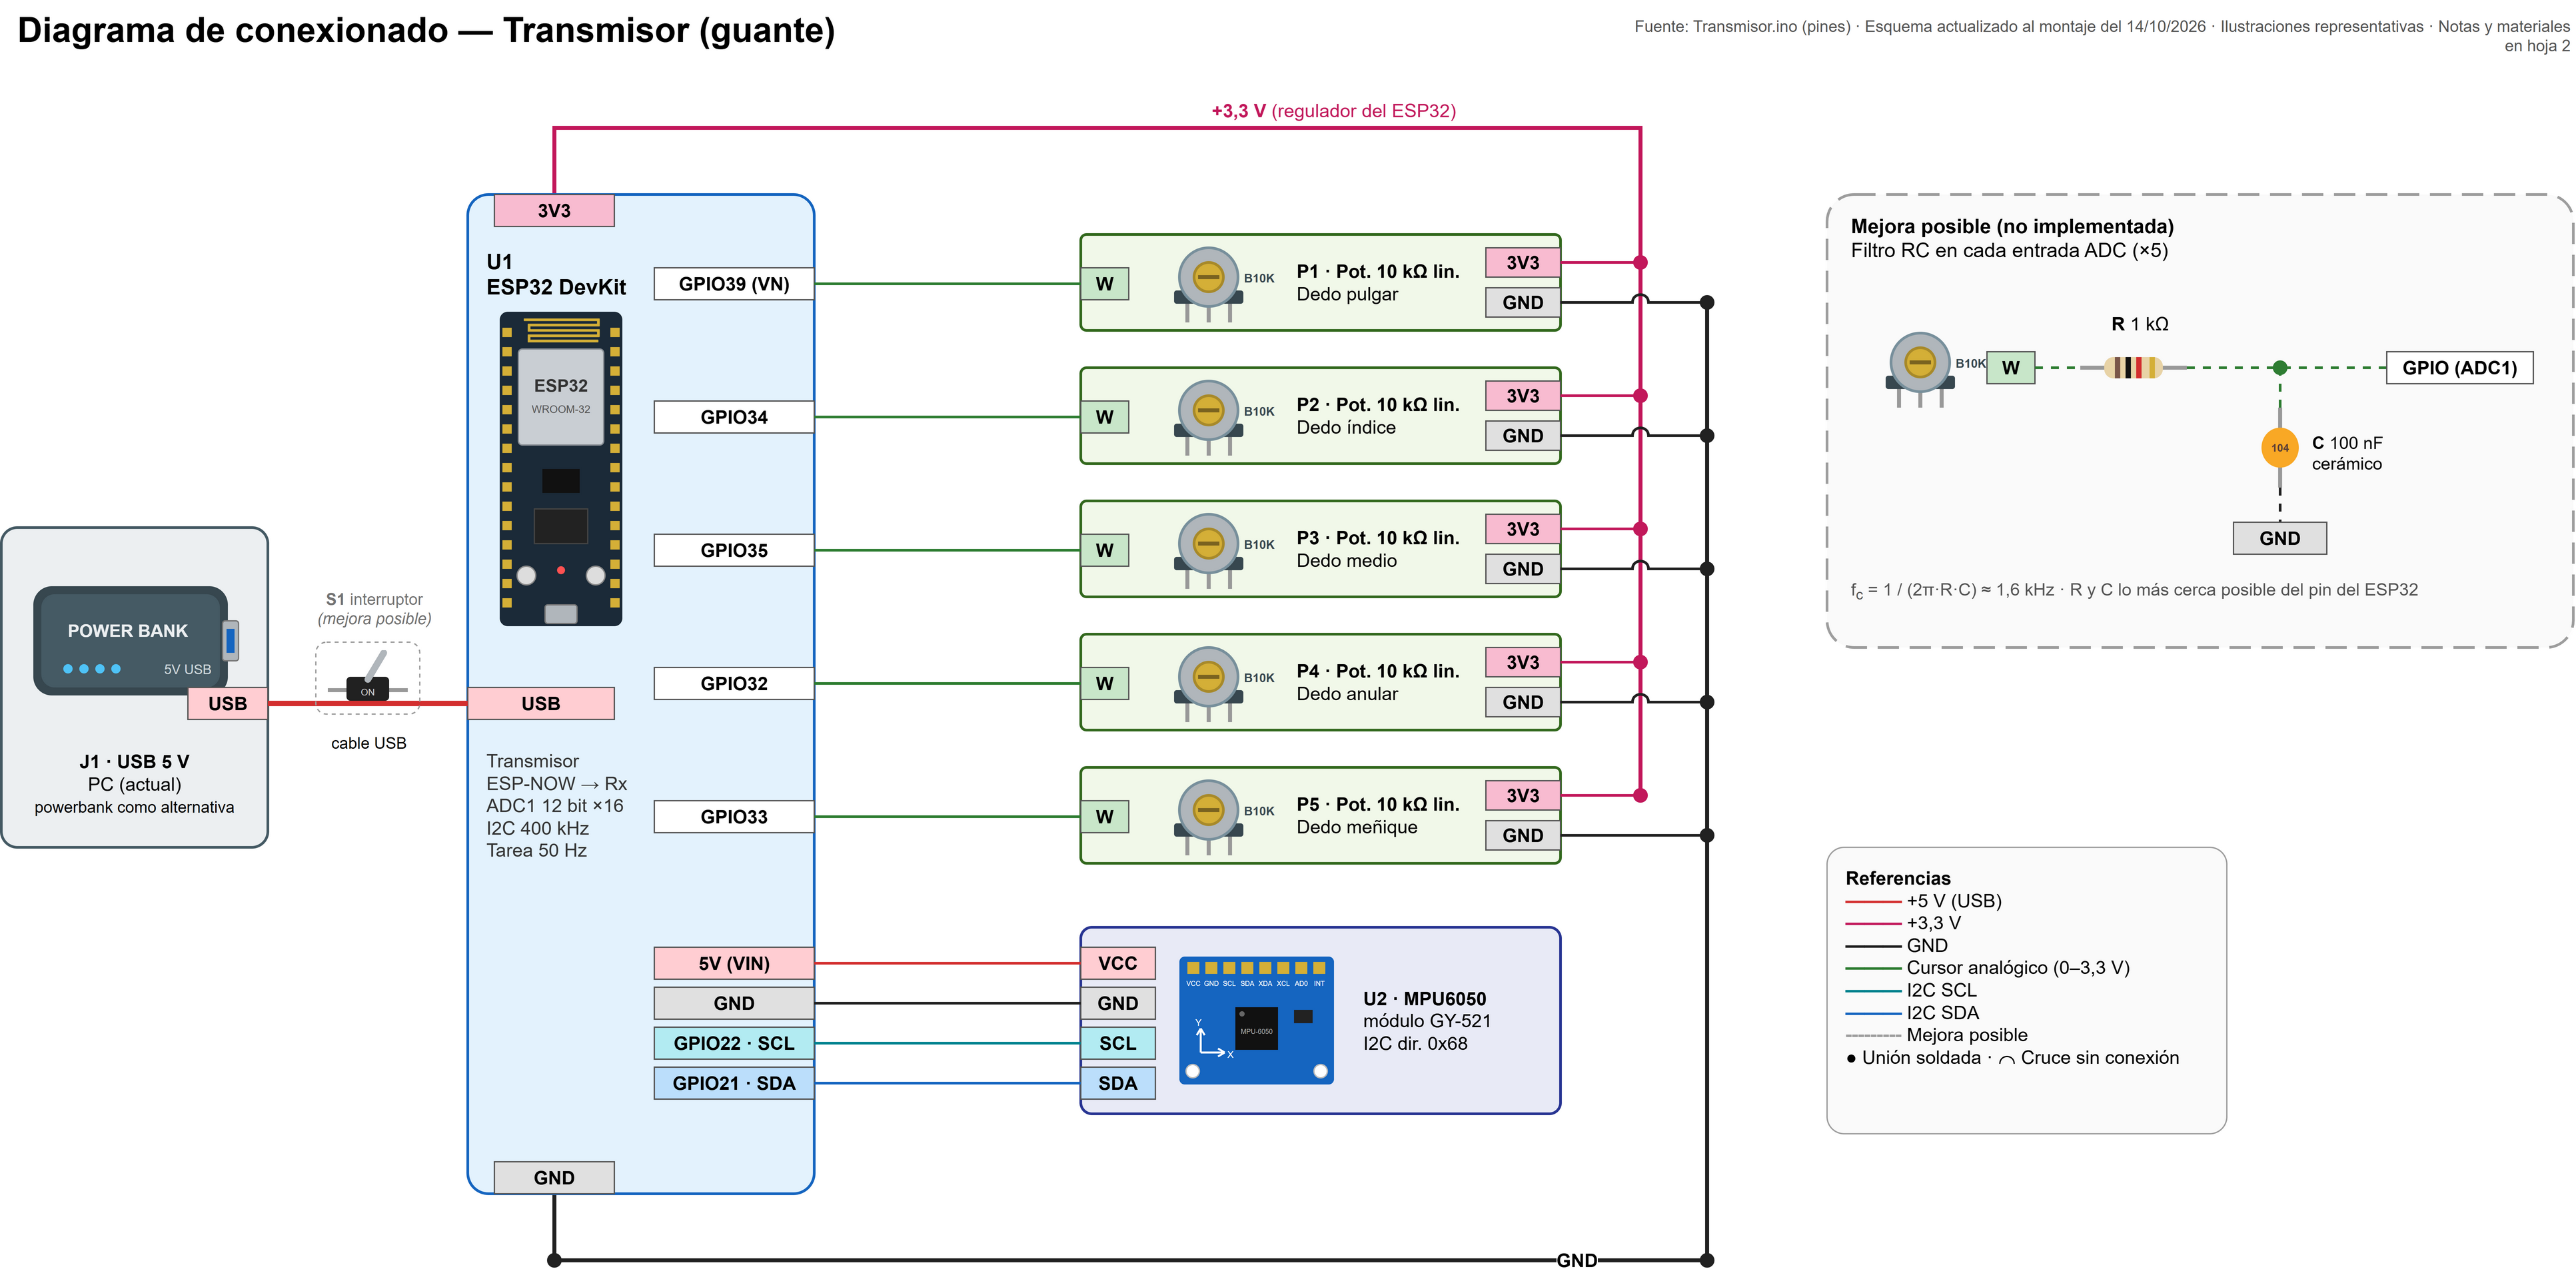
\includegraphics[width=\textwidth]{Conexionado_Transmisor_Diagrama.png}\\[0.5ex]
  \small Potenciómetros de \SI{10}{\kilo\ohm} entre \SI{3.3}{\volt} y GND, en \textbf{ADC1} (el ADC2 no funciona con la radio activa).
  El filtro RC de la derecha es una mejora posible, no implementada.
\end{frame}

%%%%%%%%%%%%%%%%%%%%%%%%%%%%%%%%%%%%%%%%%%%%%%%%%%%%%%%%%%%%%%%%%%%
\begin{frame}{Receptor: la mano robótica}
  \begin{columns}[c]
    \column{0.3\textwidth}
    \centering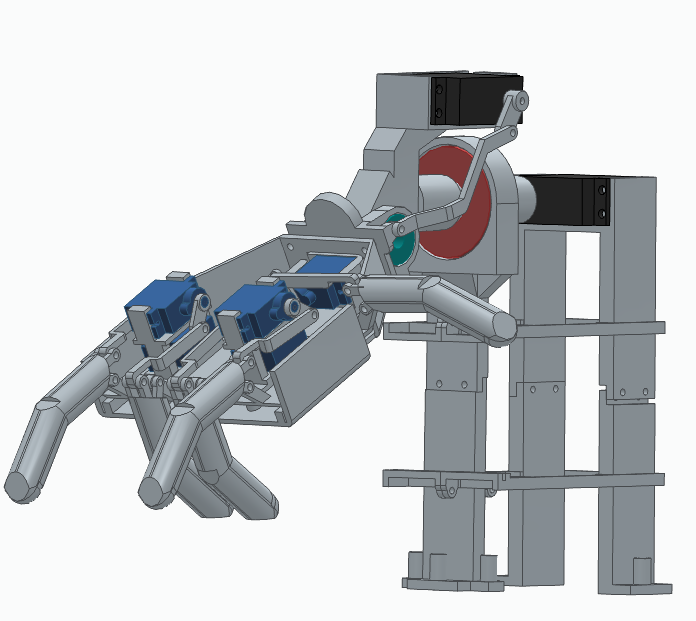
\includegraphics[width=\linewidth]{Receptor/Receptor_1.png}
    \column{0.3\textwidth}
    \centering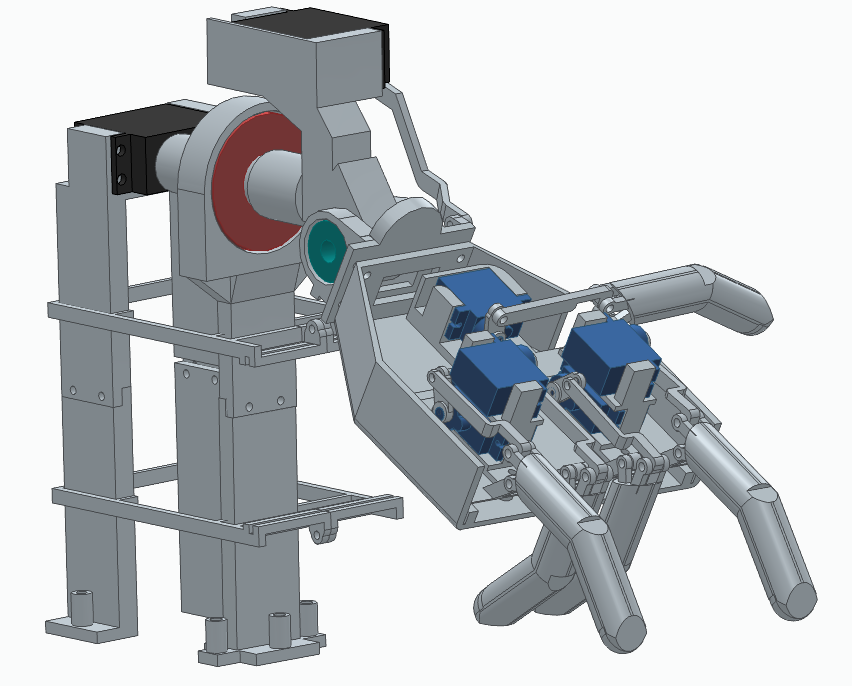
\includegraphics[width=\linewidth]{Receptor/Receptor_2.png}
    \column{0.4\textwidth}
    \begin{itemize}
      \item 5 SG90 dentro de la palma, cada uno con biela a su dedo
      \item MG946R de rotación sobre rodamiento de \SI{20}{\milli\meter}
      \item MG946R de flexión con biela en el antebrazo
      \item Recorrido mecánico mayor que el de software (\SIrange{25}{90}{\degree}): el servo nunca fuerza el plástico
      \item Impresión: Hellbot Hidra
    \end{itemize}
  \end{columns}
\end{frame}

\begin{frame}{Receptor: conexionado y alimentación}
  \centering
  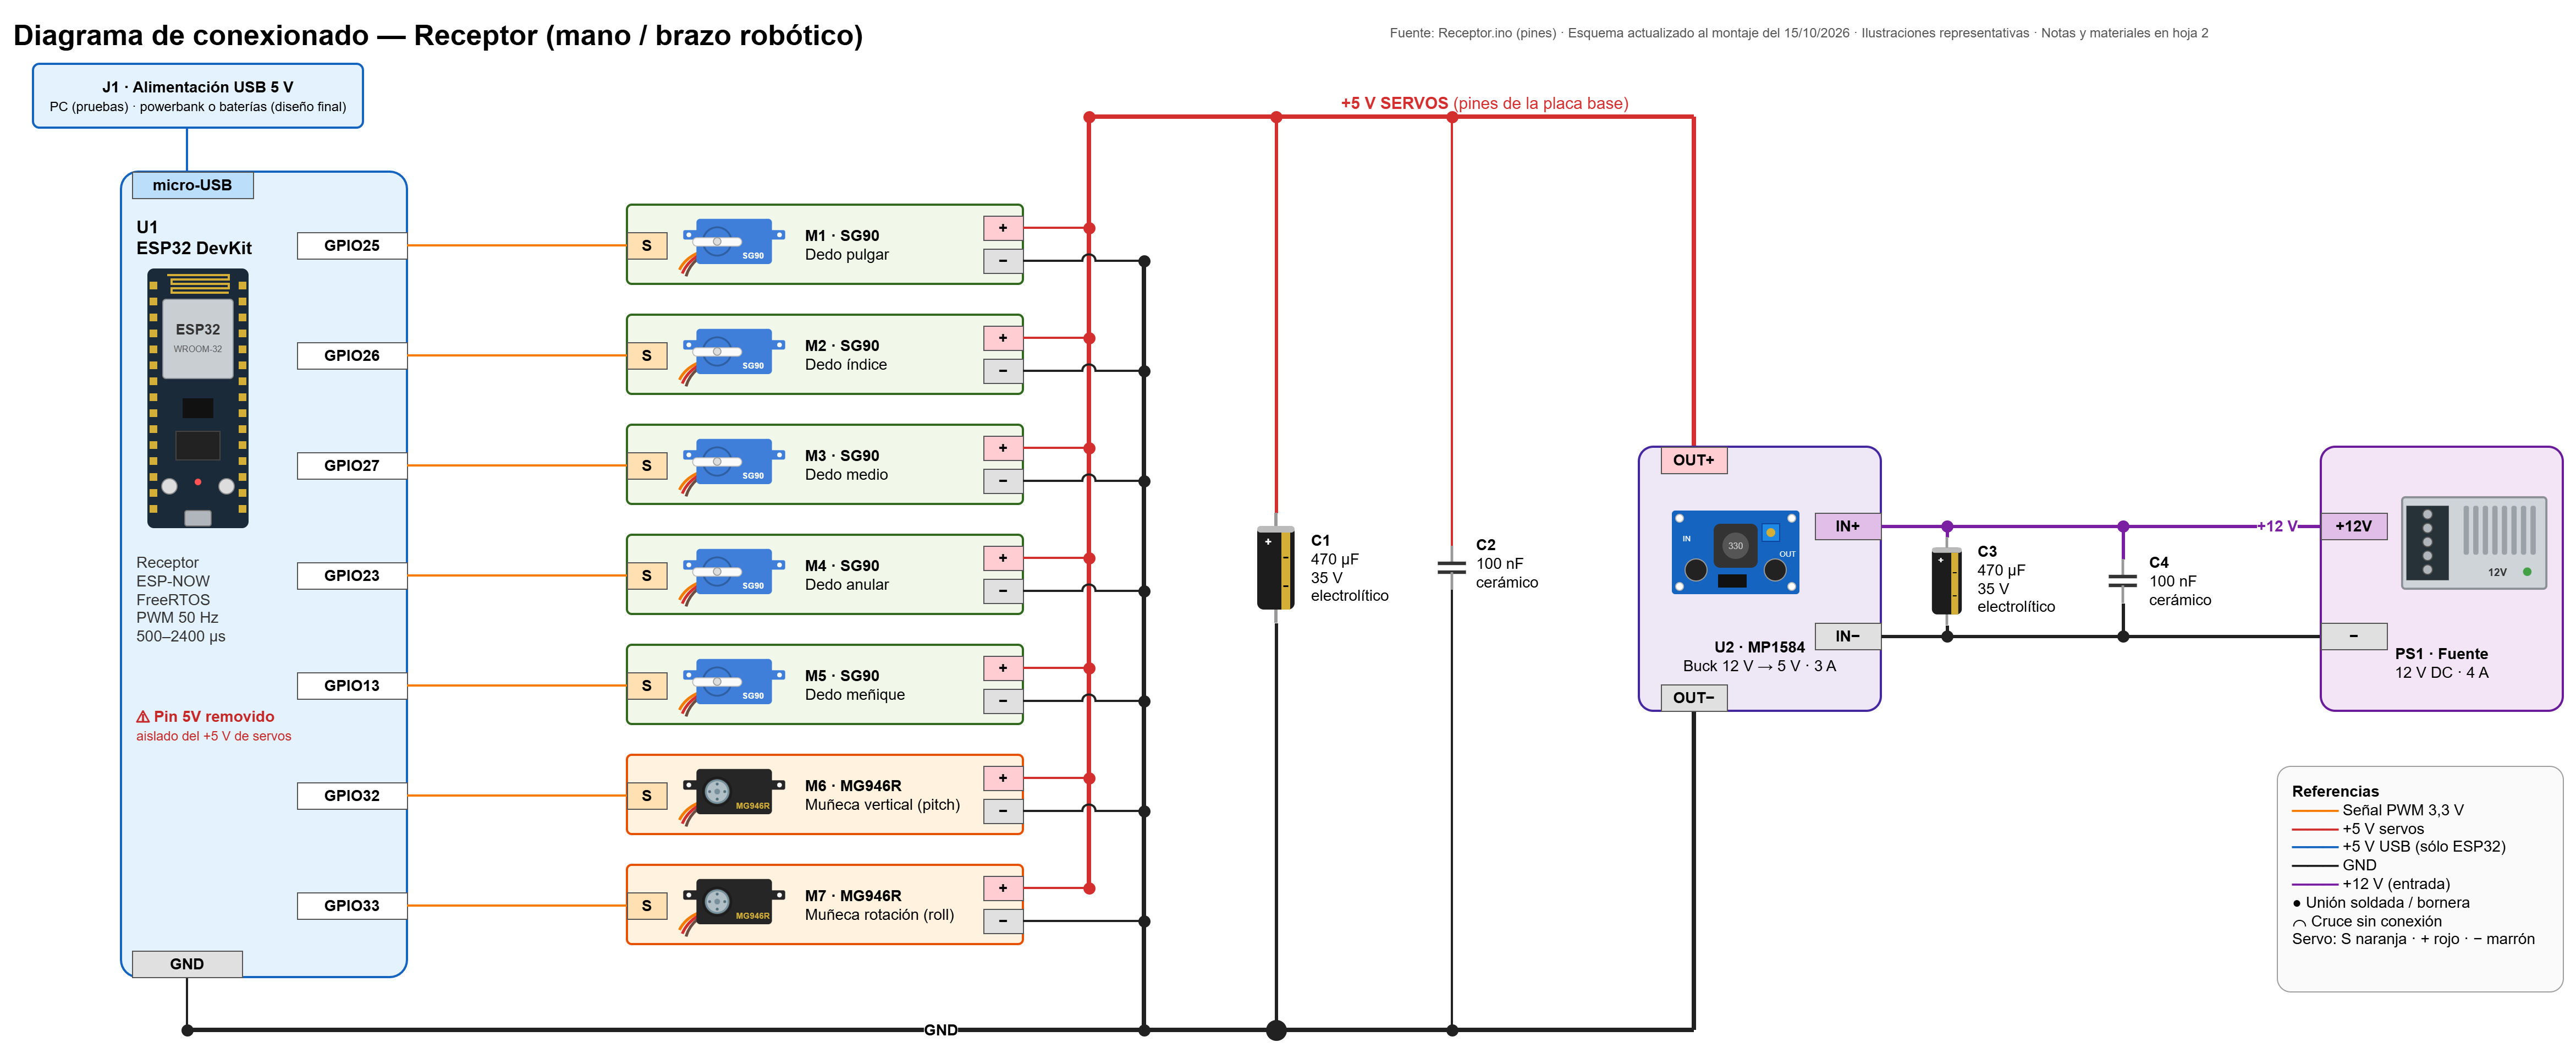
\includegraphics[width=\textwidth]{Conexionado_Receptor_Diagrama.png}\\[0.5ex]
  \begin{columns}[T]
    \column{0.5\textwidth}
    \begin{itemize}\scriptsize
      \item \textbf{Servos:} fuente \SI{12}{\volt}/\SI{4}{\ampere} $\rightarrow$ \textit{buck} MP1584 $\rightarrow$ \SI{5}{\volt}/\SI{3}{\ampere}
      \item \textbf{ESP32:} por USB, separado de los servos: un pico de los motores no lo reinicia (\textit{brownout})
    \end{itemize}
    \column{0.5\textwidth}
    \begin{itemize}\scriptsize
      \item Pin 5V del ESP32 \textbf{removido}: el regulador no inyecta corriente al USB; masas unidas
      \item \SI{470}{\micro\farad} + \SI{100}{\nano\farad} a la \textbf{entrada} y a la \textbf{salida} del regulador
    \end{itemize}
  \end{columns}
\end{frame}

%%%%%%%%%%%%%%%%%%%%%%%%%%%%%%%%%%%%%%%%%%%%%%%%%%%%%%%%%%%%%%%%%%%
\begin{frame}{Firmware en tiempo real (FreeRTOS)}
  \begin{itemize}
    \item ESP32 de dos núcleos: la pila Wi-Fi/ESP-NOW corre en el \textbf{núcleo 0}, el control en el \textbf{núcleo 1}
  \end{itemize}
  \vspace{1ex}
  \centering\small
  \begin{tabular}{l l c l}
    \toprule
    \textbf{Nodo} & \textbf{Tarea} & \textbf{Núcleo} & \textbf{Función} \\
    \midrule
    Transmisor & \texttt{tareaTransmision} & 1 & Ciclo de \SI{20}{\milli\second}: IMU, dedos, paquete, envío \\
    Transmisor & \texttt{loop()} & 1 & Consola serie (calibración) \\
    Receptor & Callback ESP-NOW & 0 & Valida y deposita en la cola \\
    Receptor & \texttt{tareaControlActuadores} & 1 & Failsafe, trayectoria, PWM \\
    \bottomrule
  \end{tabular}
  \vspace{2ex}
  \begin{itemize}
    \item Período fijo con \texttt{vTaskDelayUntil()}: no se alarga con el tiempo de cómputo (a diferencia de \texttt{delay(20)})
  \end{itemize}
\end{frame}

%%%%%%%%%%%%%%%%%%%%%%%%%%%%%%%%%%%%%%%%%%%%%%%%%%%%%%%%%%%%%%%%%%%
\begin{frame}[fragile]{Protocolo de comunicación}
  \begin{columns}[T]
    \column{0.48\textwidth}
\begin{lstlisting}
#pragma pack(push, 1)
struct MensajeBrazo {
  uint16_t magicHeader;      // 0xAA55
  uint8_t  secuencia;        // 0..255
  uint16_t anguloDedos[5];   // 25..90
  int16_t  muniecaVertical;  // 25..90
  int16_t  muniecaRotacional;// 0..180
  uint16_t checksum;         // Fletcher-16
};
#pragma pack(pop)            // 19 bytes
\end{lstlisting}
    \begin{itemize}\small
      \item ESP-NOW: sin router, por MAC, unicast con ACK
      \item \texttt{pack(1)}: sin \textit{padding}, misma disposición en ambos nodos
    \end{itemize}
    \column{0.5\textwidth}
    \textbf{Se acepta un paquete si:}
    \begin{enumerate}\small
      \item mide 19 bytes
      \item empieza con \texttt{0xAA55}
      \item el checksum coincide
    \end{enumerate}
    \vspace{1ex}
    \textbf{Fletcher-16} sobre los 17 bytes previos:
    \[
      s_1 \leftarrow (s_1 + b_i) \bmod 255, \quad s_2 \leftarrow (s_2 + s_1) \bmod 255
    \]
    \begin{itemize}\small
      \item Detecta errores de 1 bit y bytes intercambiados
      \item Sólo sumas: más simple que un CRC
      \item Segunda barrera sobre el CRC-32 de 802.11 (p.~ej. otro dispositivo ESP-NOW cercano)
    \end{itemize}
  \end{columns}
\end{frame}

%%%%%%%%%%%%%%%%%%%%%%%%%%%%%%%%%%%%%%%%%%%%%%%%%%%%%%%%%%%%%%%%%%%
\begin{frame}{Sensado de los dedos}
  \begin{columns}[T]
    \column{0.48\textwidth}
    \begin{block}{Sobremuestreo}
      Cada lectura promedia 16 conversiones del ADC:
      \[ \sigma_{\bar{x}} = \frac{\sigma}{\sqrt{N}} = \frac{\sigma}{4} \]
      Los 5 dedos en $\approx\SI{5}{\milli\second}$, dentro del ciclo de \SI{20}{\milli\second}.
    \end{block}
    \column{0.48\textwidth}
    \begin{block}{Calibración de dos puntos}
      Mano abierta ($ADC_{\min}$) y puño cerrado ($ADC_{\max}$), guardados en flash (NVS):
      \[ \theta = \operatorname{sat}_{[25,\,90]}\!\left( 25 + 65\,\frac{ADC - ADC_{\min}}{ADC_{\max} - ADC_{\min}} \right) \]
    \end{block}
  \end{columns}
  \vspace{1ex}
  \begin{itemize}
    \item La relación flexión--lectura depende de cada mano, del ajuste del guante, holguras e histéresis $\Rightarrow$ no sirve una relación fija
    \item La saturación protege la mecánica si el operador abre o cierra más que al calibrar
    \item Se calibra con \texttt{c} por consola; durante la calibración \textbf{no se transmite} (v2.3.0)
  \end{itemize}
\end{frame}

%%%%%%%%%%%%%%%%%%%%%%%%%%%%%%%%%%%%%%%%%%%%%%%%%%%%%%%%%%%%%%%%%%%
\begin{frame}{Muñeca: orientación con la IMU}
  \begin{columns}[c]
    \column{0.5\textwidth}
    \begin{itemize}
      \item \textbf{Giróscopo:} mide velocidad angular; rápido, pero al integrar el \textit{bias} el ángulo \alert{deriva}
      \item \textbf{Acelerómetro:} la gravedad da la inclinación; estable, pero \alert{ruidoso} y contaminado cuando la mano acelera
      \item Se usan \textit{pitch} (flexión) y \textit{roll} (rotación)
      \item El \textit{yaw} no se puede obtener: la gravedad no cambia al girar en torno a la vertical
    \end{itemize}
    \column{0.5\textwidth}
    \centering
    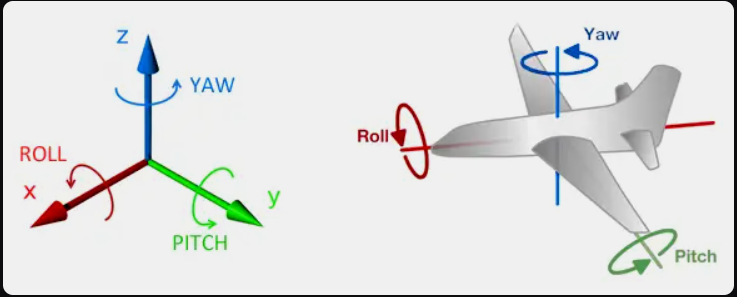
\includegraphics[width=\linewidth]{Rotaciones.png}\\[1ex]
    \[
      \phi_{acc} = \operatorname{atan2}(a_y, a_z)
    \]
    \[
      \theta_{acc} = \operatorname{atan2}\!\left(-a_x, \sqrt{a_y^2 + a_z^2}\right)
    \]
  \end{columns}
\end{frame}

\begin{frame}{Muñeca: filtro complementario}
  \[
    \theta_k = \alpha\,\underbrace{\left(\theta_{k-1} + \omega_k\,\Delta t\right)}_{\text{giróscopo: pasa-altos}}
             + (1-\alpha)\,\underbrace{\theta_{acc,k}}_{\text{acelerómetro: pasa-bajos}},
    \qquad \alpha = 0{,}98
  \]
  \[
    \tau = \frac{\alpha\,\Delta t}{1-\alpha} = \frac{0{,}98 \times \SI{0.02}{\second}}{0{,}02} \approx \SI{1}{\second}
  \]
  \begin{itemize}
    \item Movimientos más rápidos que $\tau$: manda el giróscopo (sin retardo)
    \item Tiempos mayores: el acelerómetro corrige la deriva
    \item Al encender: 500 lecturas en reposo $\rightarrow$ \textit{bias} del giróscopo y ángulo inicial
    \item Si $|\theta| \geq \SI{80}{\degree}$ el \textit{roll} se retiene (singularidad, \textit{gimbal lock})
    \item DLPF interno del MPU6050 en \SI{44}{\hertz} ($\approx\SI{5}{\milli\second}$ de retardo)
  \end{itemize}
\end{frame}

%%%%%%%%%%%%%%%%%%%%%%%%%%%%%%%%%%%%%%%%%%%%%%%%%%%%%%%%%%%%%%%%%%%
\begin{frame}{Receptor: callback, cola y tarea de control}
  \centering
  \resizebox{0.95\textwidth}{!}{%
  \begin{tikzpicture}[node distance=0.6cm and 1.5cm, every node/.style={font=\small}]
    \node[bloque] (radio) {Radio\\ESP-NOW};
    \node[bloque, right=0.8cm of radio, fill=orange!10] (cb) {Callback \texttt{OnDataRecv}\\(tarea Wi-Fi, núcleo 0)\\Valida tamaño,\\firma y checksum};
    \node[bloque, right=of cb, fill=yellow!15] (cola) {Cola\\(1 elemento)};
    \node[bloque, right=of cola, fill=green!10] (ctrl) {Tarea de control\\(núcleo 1)\\Failsafe, trayectoria\\y escritura PWM};
    \node[bloque, right=0.8cm of ctrl] (servos) {7 servos};
    \draw[flecha] (radio) -- (cb);
    \draw[flecha] (cb) -- node[below, font=\footnotesize]{sobrescribe} (cola);
    \draw[flecha] (cola) -- node[below, font=\footnotesize]{despierta} (ctrl);
    \draw[flecha] (ctrl) -- (servos);
  \end{tikzpicture}}
  \vspace{2ex}
  \begin{itemize}
    \item \textbf{Cola de 1 elemento} con \texttt{xQueueOverwrite}: copia atómica (sin condición de carrera) y buzón del \emph{último} paquete (sin retardo acumulado)
    \item La tarea \textbf{despierta al llegar el paquete} (v2.2.0); si no llega, vence a los \SI{20}{\milli\second} e itera igual
    \item Objetivos saturados a los límites mecánicos: segunda protección ante valores fuera de rango
  \end{itemize}
\end{frame}

\begin{frame}{Receptor: máquina de estados y failsafe}
  \centering
  \resizebox{0.85\textwidth}{!}{%
  \begin{tikzpicture}[node distance=1.6cm and 2.2cm, every node/.style={font=\small},
    estado/.style={draw, rounded corners=8pt, align=center, minimum width=3cm, minimum height=1.1cm, fill=blue!5}]
    \node[estado] (sync) {\texttt{ESPERANDO\_SYNC}\\Servos en reposo};
    \node[estado, right=of sync, fill=green!10] (normal) {\texttt{OPERACION\_NORMAL}\\Sigue al guante};
    \node[estado, below=of normal, fill=red!10] (fs) {\texttt{FAILSAFE\_SIN\_SENAL}\\Objetivos en reposo};
    \node[estado, right=of fs, fill=gray!15, dashed] (desac) {Servos desacoplados\\(sin PWM)};
    \draw[flecha] ($(sync.north)+(0,0.7)$) -- node[right, font=\footnotesize]{Inicio} (sync);
    \draw[flecha] (sync) -- node[above, font=\footnotesize]{Paquete válido} (normal);
    \draw[flecha] ($(normal.south)+(0.5,0)$) -- node[right, font=\footnotesize, align=left]{$>\SI{250}{\milli\second}$\\sin paquetes} ($(fs.north)+(0.5,0)$);
    \draw[flecha] ($(fs.north)+(-0.5,0)$) -- node[left, font=\footnotesize]{Paquete válido} ($(normal.south)+(-0.5,0)$);
    \draw[flecha] (fs) -- node[above, font=\footnotesize, align=center]{En reposo y\\$>\SI{2}{\second}$} (desac);
    \draw[flecha] (desac.north) |- node[pos=0.25, right, font=\footnotesize, align=left]{Paquete válido\\(reacopla)} (normal.east);
  \end{tikzpicture}}
  \begin{itemize}\small
    \item \SI{250}{\milli\second} $\approx$ 12 paquetes perdidos: tolera interferencias breves, reacciona rápido ante un corte real
    \item Sin PWM los servos dejan de consumir y de calentarse; al volver arrancan desde la última posición (sin salto)
  \end{itemize}
\end{frame}

%%%%%%%%%%%%%%%%%%%%%%%%%%%%%%%%%%%%%%%%%%%%%%%%%%%%%%%%%%%%%%%%%%%
\begin{frame}{Suavizado: limitador de velocidad y banda muerta}
  \[
    e_i[k] = \theta^{obj}_i - \theta_i[k-1], \qquad
    \theta_i[k] =
    \begin{cases}
      \theta_i[k-1] + \operatorname{sat}_{\pm\Delta\theta_{\max}}\!\left(e_i[k]\right) & |e_i[k]| > \delta \\
      \theta_i[k-1] & |e_i[k]| \leq \delta
    \end{cases}
  \]
  \begin{columns}[T]
    \column{0.5\textwidth}
    \begin{itemize}\small
      \item \textbf{Limitador:} un salto grande (reconexión, failsafe) se vuelve rampa $\Rightarrow$ menos picos de corriente y esfuerzo mecánico
      \item \textbf{Banda muerta:} evita que el servo corrija décimas de grado y zumbe (\textit{hunting})
      \item Límites cercanos a la velocidad del servo: en uso normal casi no agregan retardo
    \end{itemize}
    \column{0.5\textwidth}
    \centering\small
    \begin{tabular}{l c c}
      \toprule
      \textbf{Servo} & \textbf{Vel. máx.} & $\boldsymbol{\delta}$ \\
      \midrule
      Dedos (SG90) & \SI{400}{\degree\per\second} & \SI{1.0}{\degree} \\
      Muñeca vertical & \SI{200}{\degree\per\second} & \SI{1.2}{\degree} \\
      Muñeca rotación & \SI{250}{\degree\per\second} & \SI{1.2}{\degree} \\
      \bottomrule
    \end{tabular}\\
    {\scriptsize Ciclo de \SI{20}{\milli\second}: 8°, 4° y 5° por ciclo}
  \end{columns}
\end{frame}

%%%%%%%%%%%%%%%%%%%%%%%%%%%%%%%%%%%%%%%%%%%%%%%%%%%%%%%%%%%%%%%%%%%
\begin{frame}{Evolución del diseño: cada cambio, un problema observado}
  \centering\small
  \begin{tabular}{l p{6.2cm} p{4.6cm}}
    \toprule
    \textbf{Versión} & \textbf{Cambio} & \textbf{Motivo} \\
    \midrule
    Preliminar & EMA en guante y mano, \texttt{delay(20)}, lecturas crudas & Primera versión funcional \\
    1.0.0 & FreeRTOS, cola, checksum, limitador, NVS, \textbf{Kalman} & Retardo y zumbido \\
    2.0.0 & \textbf{Filtro complementario}, calibración del giróscopo & Muñeca derivaba ``como un mouse'' \\
    2.1.0 & Limitador más rápido, inversión de dedos & Respuesta lenta, dedos invertidos \\
    2.2.0 & Receptor actúa al llegar el paquete, DLPF \SI{44}{\hertz} & Reducir latencia \\
    2.3.0 & Sin transmisión durante la calibración & Mano imitaba la calibración \\
    \bottomrule
  \end{tabular}
  \vspace{1.5ex}
  \begin{itemize}\small
    \item \textbf{v2.3.0: versión definitiva, probada en hardware}
    \item Cada versión es un \textit{tag} de git: cualquiera se puede reproducir y comparar
    \item Doble EMA: los retardos se suman, y los pasos cada vez más chicos caen en la zona muerta del servo $\Rightarrow$ zumbido
  \end{itemize}
\end{frame}

\begin{frame}{¿Por qué complementario y no Kalman?}
  \begin{columns}[T]
    \column{0.5\textwidth}
    \textbf{Lo que se encontró en la v1.0.0}
    \begin{enumerate}\small
      \item Signo del giróscopo de \textit{pitch} invertido: giróscopo y acelerómetro tiraban en sentidos opuestos
      \item Variable sin inicializar en el \textit{roll}
      \item Arranque desde \SI{0}{\degree}, sin estimar el \textit{bias}
      \item Truncado a enteros antes del mapeo
    \end{enumerate}
    \column{0.5\textwidth}
    \textbf{Por qué se cambió el filtro}
    \begin{itemize}\small
      \item Un Kalman bien sintonizado \alert{no es peor}
      \item Pero para 2 ángulos de inclinación a \SI{50}{\hertz} el complementario es equivalente en la práctica
      \item \textbf{Un parámetro} ($\alpha$) con interpretación directa ($\tau \approx \SI{1}{\second}$), en lugar de 3 covarianzas
      \item Más fácil de verificar
    \end{itemize}
  \end{columns}
\end{frame}

%%%%%%%%%%%%%%%%%%%%%%%%%%%%%%%%%%%%%%%%%%%%%%%%%%%%%%%%%%%%%%%%%%%
\begin{frame}{Latencia}
  \begin{columns}[T]
    \column{0.58\textwidth}
    \textbf{Estimación} (código y hojas de datos)\\[0.5ex]
    \scriptsize
    \begin{tabular}{l c}
      \toprule
      \textbf{Etapa} & \textbf{Retardo} \\
      \midrule
      Espera al ciclo del transmisor & 0--\SI{20}{\milli\second} (media 10) \\
      DLPF del MPU6050 (muñeca) & $\approx\SI{5}{\milli\second}$ \\
      Lectura de dedos y cálculo & $\approx\SI{5}{\milli\second}$ \\
      Transmisión ESP-NOW & 1--\SI{6}{\milli\second} \\
      Tarea de control del receptor & $<\SI{1}{\milli\second}$ \\
      Siguiente pulso PWM & 0--\SI{20}{\milli\second} (media 10) \\
      \midrule
      \textbf{Hasta la orden al servo} & $\boldsymbol{\approx\SI{30}{\milli\second}}$ \textbf{media} \\
      \bottomrule
    \end{tabular}\\[0.5ex]
    \small + movimiento mecánico ($\approx\SI{0.1}{\second}$ cada \SI{60}{\degree} en el SG90)
    \column{0.4\textwidth}
    \textbf{Medición por cable}
    \begin{itemize}\small
      \item GPIO23 del transmisor marca el inicio de cada ciclo
      \item El receptor captura el flanco por interrupción (GPIO34)
      \item Por paquete: tiempo de radio y total
      \item Sin osciloscopio; estadística en MATLAB
    \end{itemize}
    \vspace{1ex}
    \pendiente{medición en curso: completar con media, máximo e histograma (P11)}
  \end{columns}
\end{frame}

%%%%%%%%%%%%%%%%%%%%%%%%%%%%%%%%%%%%%%%%%%%%%%%%%%%%%%%%%%%%%%%%%%%
\begin{frame}{Respuesta del sistema (v2.3.0)}
  \begin{columns}[T]
    \column{0.36\textwidth}
    \centering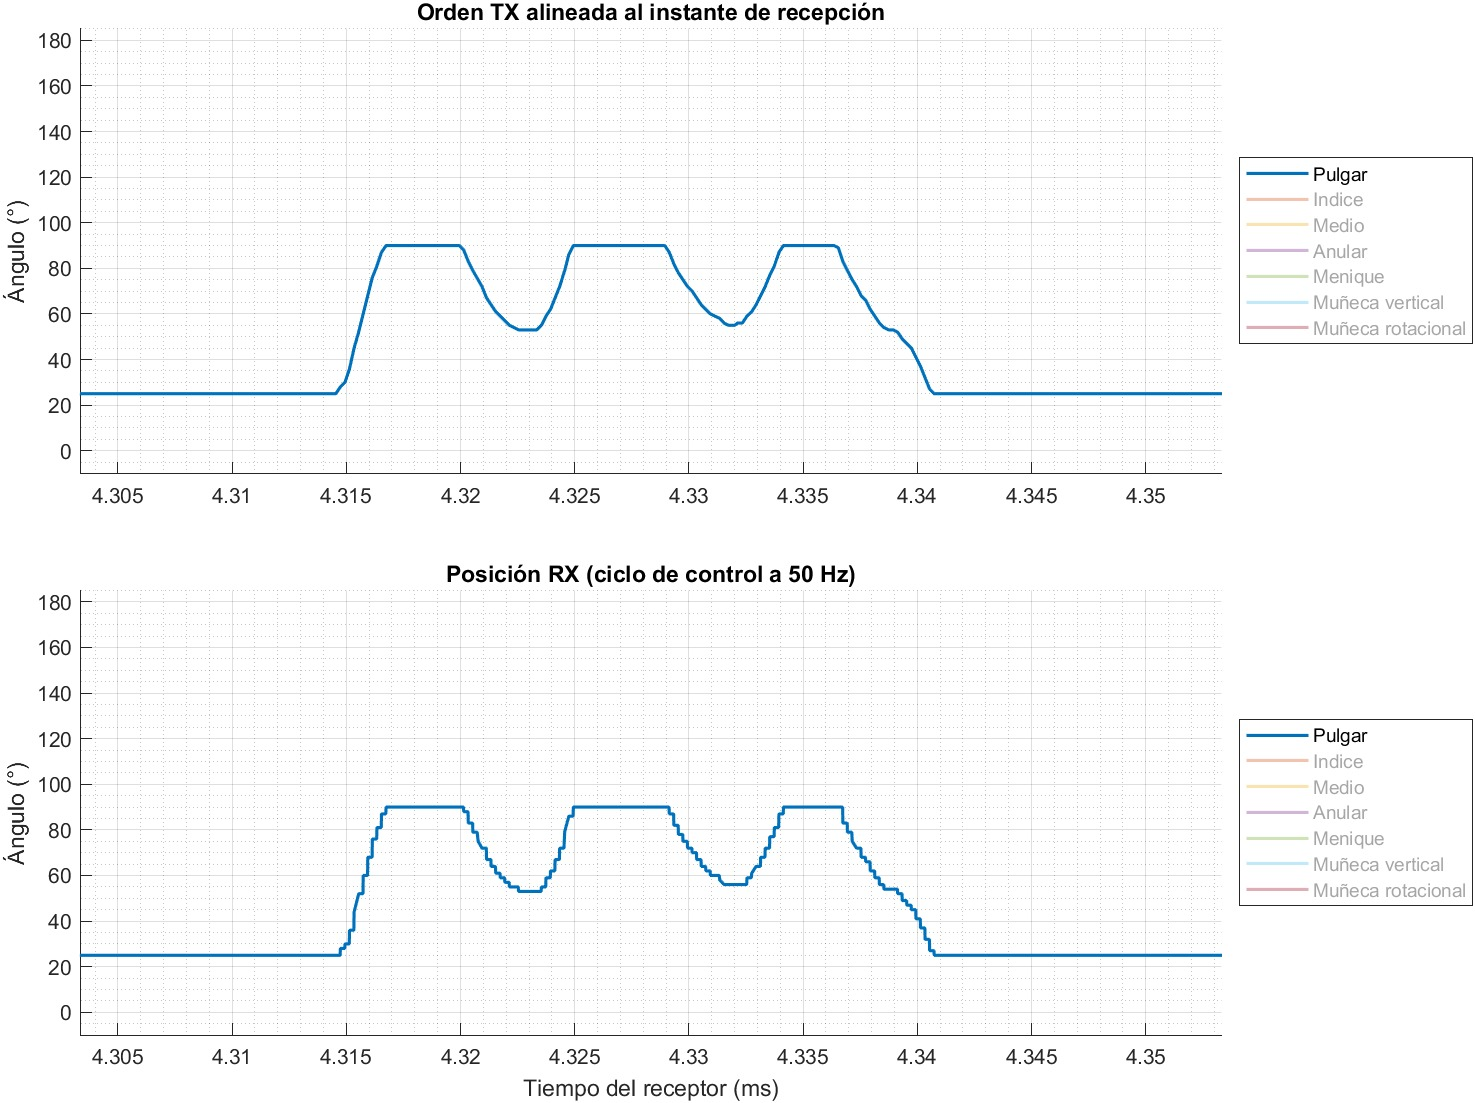
\includegraphics[width=\linewidth]{Mediciones/P16_matlab_pulgar.jpg}\\{\scriptsize Pulgar}
    \column{0.36\textwidth}
    \centering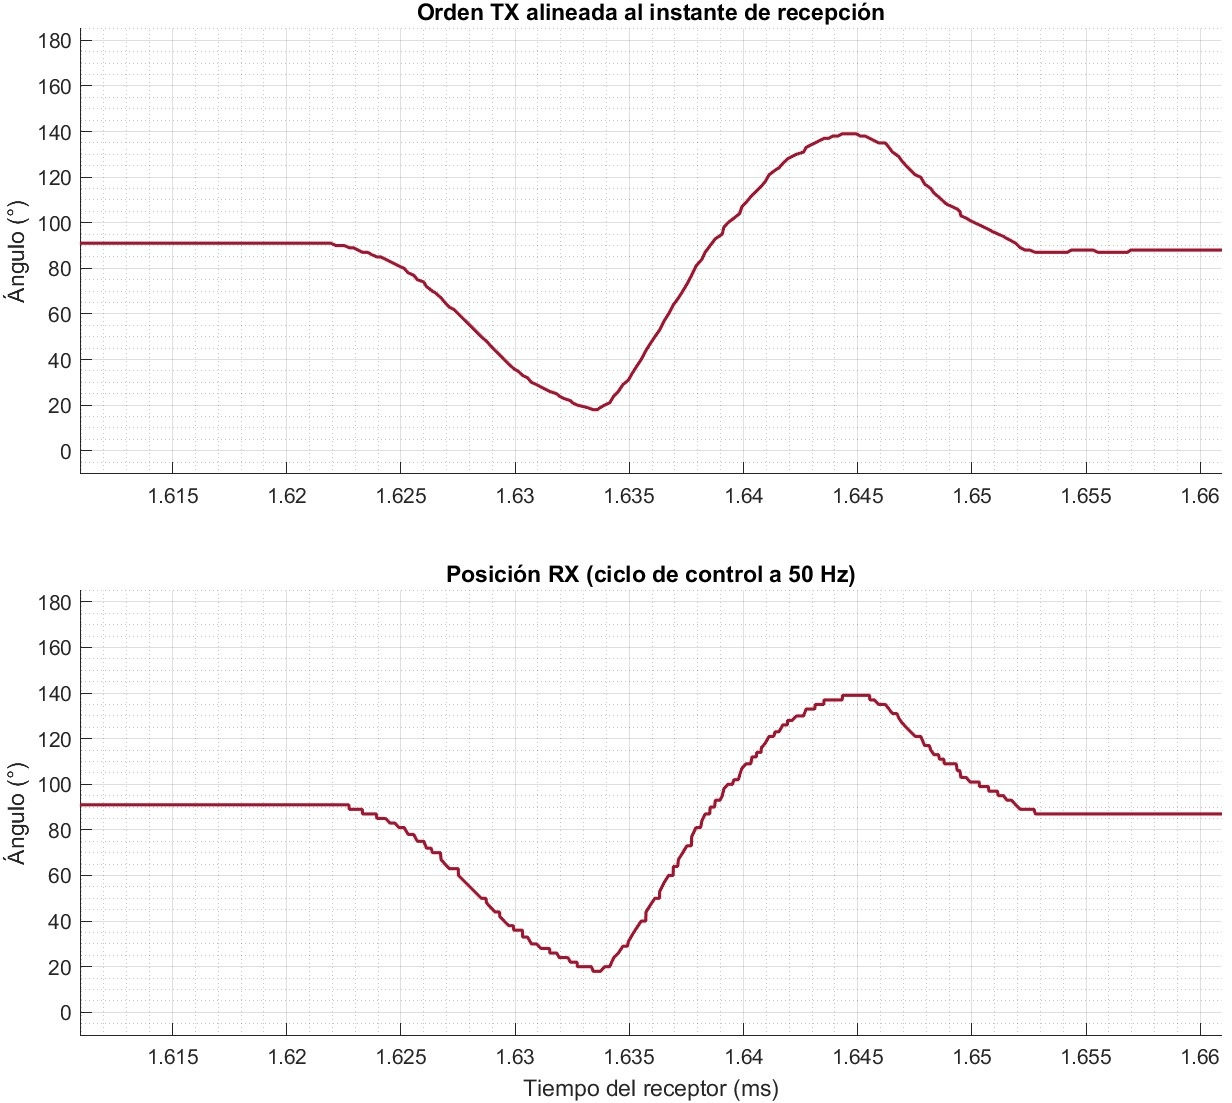
\includegraphics[width=\linewidth]{Mediciones/P16_matlab_muneca_rotacional.jpg}\\{\scriptsize Muñeca rotacional}
    \column{0.28\textwidth}
    \scriptsize
    Arriba: orden del guante. Abajo: posición aplicada por la mano.\\[1ex]
    \textbf{Alineación por número de secuencia}: telemetría CSV a \SI{50}{\hertz} de ambos nodos, ubicada en el reloj del receptor.\\[1ex]
    El corrimiento muestra el limitador y la banda muerta, \alert{no la latencia del enlace}.\\[1ex]
    {\tiny Eje: \SI{500}{\milli\second}/div (el factor $\times10^5$ de MATLAB quedó fuera de la captura).}
  \end{columns}
  \vspace{1ex}
  \begin{itemize}\small
    \item \textbf{Seguimiento} de la forma completa y de posiciones intermedias (índice en $\approx$\SI{57}{\degree} y \SI{46}{\degree}); sin retraso visible a esta escala
    \item \textbf{Saturación} en \SIrange{25}{90}{\degree}; pasos de la orden menores que el límite del limitador $\Rightarrow$ sigue paquete a paquete
    \item \textbf{Banda muerta:} las variaciones de \SI{1}{\degree} en las mesetas no llegan al servo (error final $\leq$ \SI{1}{\degree})
  \end{itemize}
\end{frame}

\begin{frame}{Consumo del receptor (v2.3.0)}
  \begin{columns}[T]
    \column{0.33\textwidth}
    \centering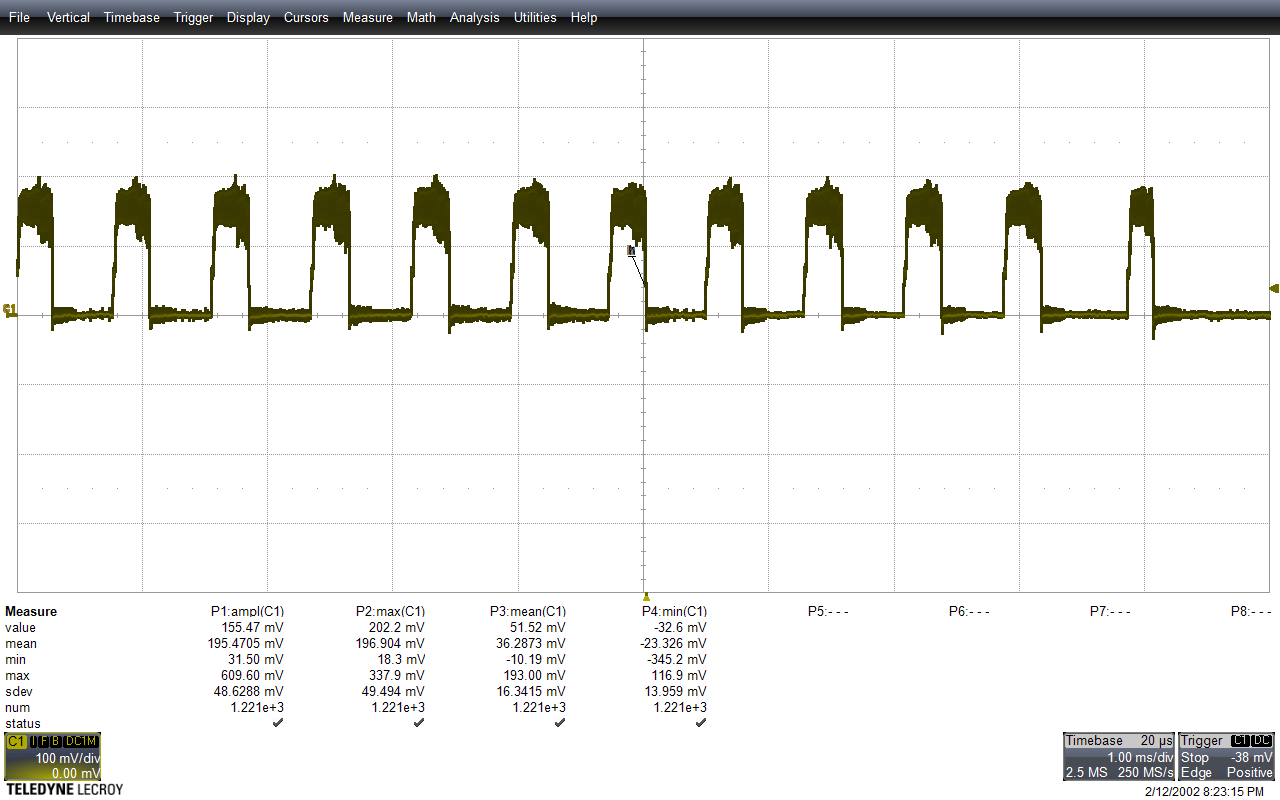
\includegraphics[width=\linewidth]{Mediciones/P02_reposo_sin_cap_entrada.png}\\{\scriptsize Reposo, sin capacitor de entrada}
    \column{0.33\textwidth}
    \centering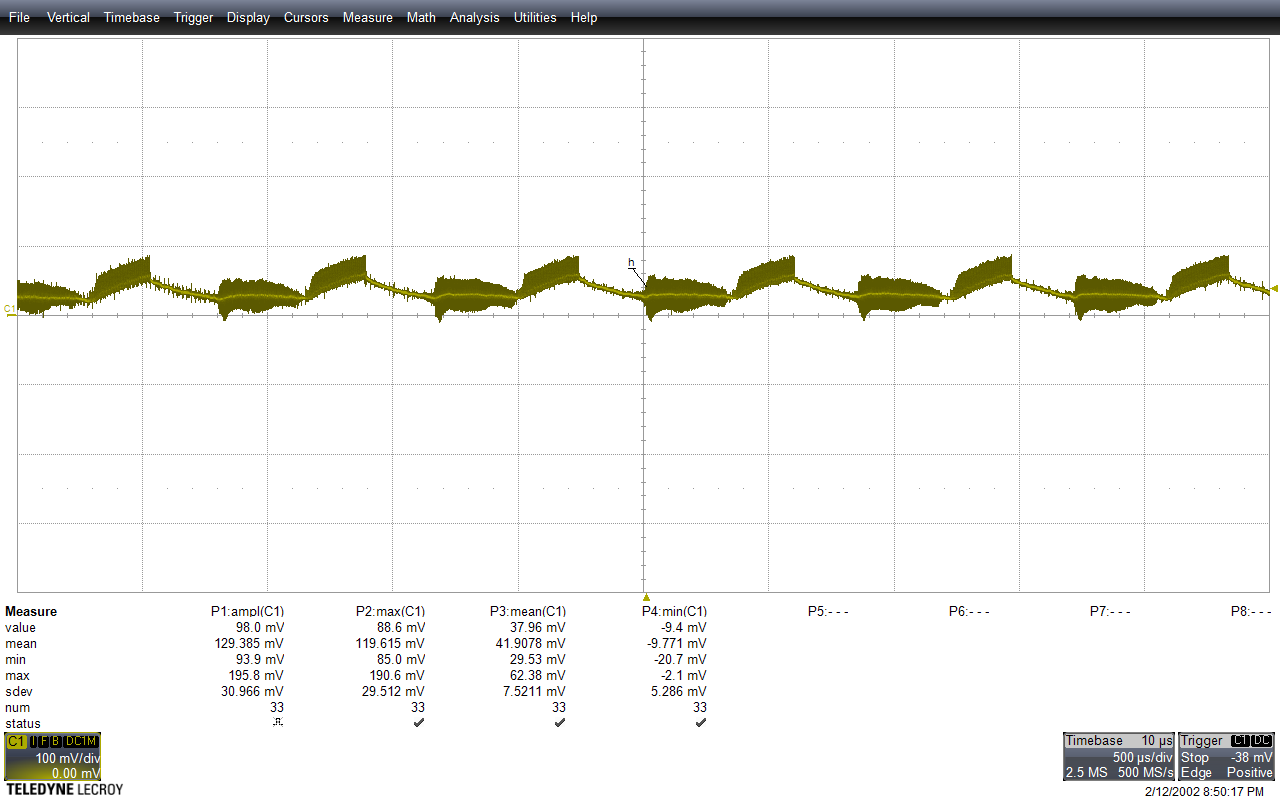
\includegraphics[width=\linewidth]{Mediciones/P02_reposo_con_cap_entrada.png}\\{\scriptsize Reposo, con capacitor de entrada}
    \column{0.33\textwidth}
    \centering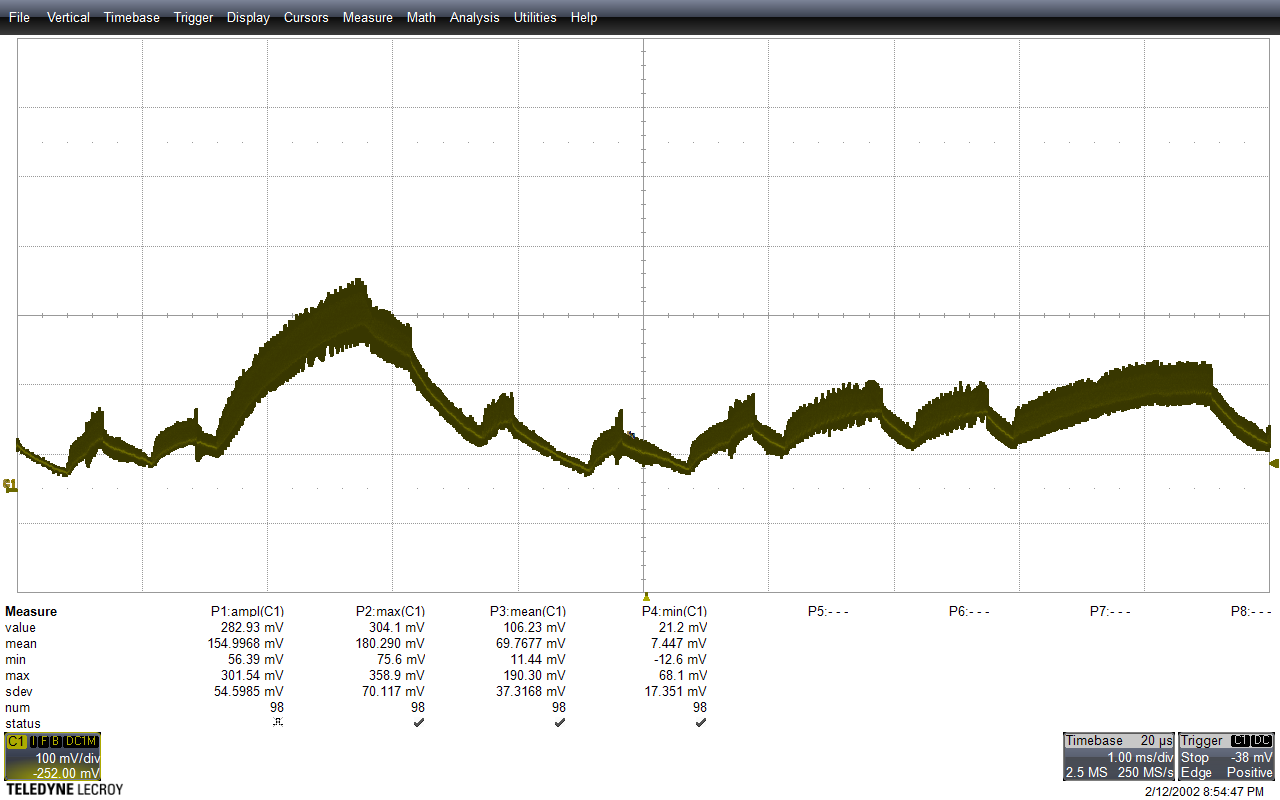
\includegraphics[width=\linewidth]{Mediciones/P03_pitch_roll_con_cap.png}\\{\scriptsize \textit{Pitch} y \textit{roll} simultáneos}
  \end{columns}
  \vspace{1ex}
  \begin{columns}[T]
    \column{0.5\textwidth}
    \centering\scriptsize
    \begin{tabular}{l c}
      \toprule
      \textbf{Situación} (a \SI{12}{\volt}) & \textbf{Corriente} \\
      \midrule
      Reposo (media) & \SIrange{75}{100}{\milli\ampere} \\
      Muñeca en 2 ejes (media / picos) & \SI{0.21}{\ampere} / \SIrange{0.6}{0.72}{\ampere} \\
      Servo bloqueado a mano & \SIrange{0.55}{0.6}{\ampere} \\
      \bottomrule
    \end{tabular}
    \column{0.5\textwidth}
    \begin{itemize}\scriptsize
      \item Shunt de \SI{0.5}{\ohm} en el negativo de \SI{12}{\volt}, osciloscopio LeCroy
      \item Pulsos en reposo: \textit{pulse-skipping} del MP1584 (normal)
      \item Capacitor de entrada: pico de \SI{0.38}{\ampere} $\rightarrow$ \SI{0.18}{\ampere}, misma media
      \item Salida de \SI{5}{\volt}: \SIrange{5.14}{5.25}{\volt}, variación imperceptible
      \item Peor caso $<\SI{0.75}{\ampere}$: muy por debajo de \SI{4}{\ampere} (fuente) y \SI{3}{\ampere} (regulador)
    \end{itemize}
  \end{columns}
\end{frame}

\begin{frame}{Resumen de pruebas (v2.3.0)}
  \centering\small
  \begin{tabular}{l l c}
    \toprule
    \textbf{Prueba} & \textbf{Resultado} & \\
    \midrule
    Consumo en reposo y con carga (P02, P03) & \SI{75}{\milli\ampere} a \SI{0.72}{\ampere} a \SI{12}{\volt} & \checkmark \\
    Tensión de \SI{5}{\volt} de los servos (P04) & Variación imperceptible & \checkmark \\
    Calibración sin transmisión (P09) & La mano va a reposo y se recupera & \checkmark \\
    Respuesta del sistema con MATLAB (P16) & Seguimiento en dedos y muñeca & \checkmark \\
    \midrule
    Latencia de punta a punta (P11) & \pendiente{medición por cable en curso} & \\
    Muñeca: deriva y retorno a la posición (P13) & \pendiente{a realizar} & \\
    Failsafe al apagar el guante (P10) & \pendiente{registrar} & \\
    \bottomrule
  \end{tabular}
\end{frame}

%%%%%%%%%%%%%%%%%%%%%%%%%%%%%%%%%%%%%%%%%%%%%%%%%%%%%%%%%%%%%%%%%%%
\begin{frame}{Conclusiones}
  \begin{itemize}
    \item Telerobótica de bajo costo: se replican los 5 dedos y 2 grados de libertad de la muñeca por ESP-NOW; con la v2.3.0 la mano sigue la orden, incluidas las posiciones intermedias
    \item \textbf{Separación de responsabilidades:} el guante calcula, la mano valida, suaviza y mueve
    \item \textbf{Seguridad en el firmware:} checksum, failsafe a \SI{250}{\milli\second}, límites mecánicos, rampa de velocidad
    \item \textbf{Diseño iterativo validado en hardware:} 6 versiones, cada cambio con un motivo observado; el filtrado doble sumaba retardo y un filtro simple y verificable resolvió la deriva
    \item \textbf{Alimentación:} consumo medido muy por debajo de la capacidad; ESP32 separado de los servos
    \item Limitaciones: sin realimentación de fuerza, \textit{yaw} no medido (sin magnetómetro), depende de la calibración
  \end{itemize}
\end{frame}

\begin{frame}{Trabajo futuro}
  \begin{itemize}
    \item \textbf{Medir la latencia real} de punta a punta (en curso, método por cable)
    \item Repetir la deriva y el retorno de la muñeca con la v2.3.0
    \item \textbf{Subir las frecuencias:} envío a \SI{100}{\hertz} (escalando el limitador con el $\Delta t$ real) y PWM de \SIrange{100}{200}{\hertz} en los MG946R, vigilando temperatura
    \item Filtro RC en las entradas del ADC del guante
    \item Realimentación háptica al operador
  \end{itemize}
\end{frame}

\begin{frame}[plain]
  \centering\vfill
  {\Huge\color{unsazul}\textbf{¡Gracias!}}\\[3ex]
  {\Large Preguntas}\\[4ex]
  \small Joaquín Petruf \quad Sebastián Amoroso
  \vfill
\end{frame}

%%%%%%%%%%%%%%%%%%%%%%%%%%%%%%%%%%%%%%%%%%%%%%%%%%%%%%%%%%%%%%%%%%%
% RESPALDO: para preguntas del jurado (no se exponen)
\appendix

\begin{frame}{Respaldo: filtro de Kalman (v1.0.0)}
  Estado: ángulo $\theta$ y \textit{bias} del giróscopo $b$
  \[
    \text{Predicción:}\quad \theta^- = \theta + \Delta t\,(\omega - b), \qquad P^- = F P F^{T} + Q\,\Delta t,
    \qquad F = \begin{pmatrix} 1 & -\Delta t \\ 0 & 1 \end{pmatrix}
  \]
  \[
    \text{Corrección:}\quad K = \frac{1}{P^-_{00} + R}\begin{pmatrix} P^-_{00} \\ P^-_{10} \end{pmatrix}, \qquad
    \begin{pmatrix} \theta \\ b \end{pmatrix} \leftarrow \begin{pmatrix} \theta^- \\ b \end{pmatrix} + K\left(\theta_{acc} - \theta^-\right)
  \]
  \[
    Q_{angle} = 0{,}001, \quad Q_{bias} = 0{,}003, \quad R = 0{,}03
  \]
  \begin{itemize}\small
    \item Tres parámetros sin interpretación directa frente a un único $\alpha$
    \item El problema real eran errores de signo e inicialización, no el filtro
  \end{itemize}
\end{frame}

\begin{frame}{Respaldo: mapeo de la muñeca}
  \textit{Pitch} en dos tramos (rango del operador \SI{+45}{\degree}/\SI{-25}{\degree}, neutro del servo en \SI{57}{\degree}):
  \[
    \theta_{servo,V} =
    \begin{cases}
      57 - \dfrac{p}{45}\,(57 - 25) & p \geq 0 \\[1.5ex]
      57 + \dfrac{p}{-25}\,(90 - 57) & p < 0
    \end{cases}
    \qquad p = \operatorname{sat}_{[-25,\,45]}\left(\theta - \theta_{trim}\right)
  \]
  Rotación lineal, mano plana = servo centrado:
  \[
    \theta_{servo,R} = \operatorname{sat}_{[0,\,180]}\left(\phi - \phi_{trim} + 90\right)
  \]
  \begin{itemize}\small
    \item $\theta_{trim}$, $\phi_{trim}$ compensan la desalineación de montaje del MPU6050
    \item Cálculo en punto flotante, redondeo al grado al empaquetar
  \end{itemize}
\end{frame}

\begin{frame}{Respaldo: respuesta del índice y de la muñeca vertical}
  \begin{columns}[T]
    \column{0.5\textwidth}
    \centering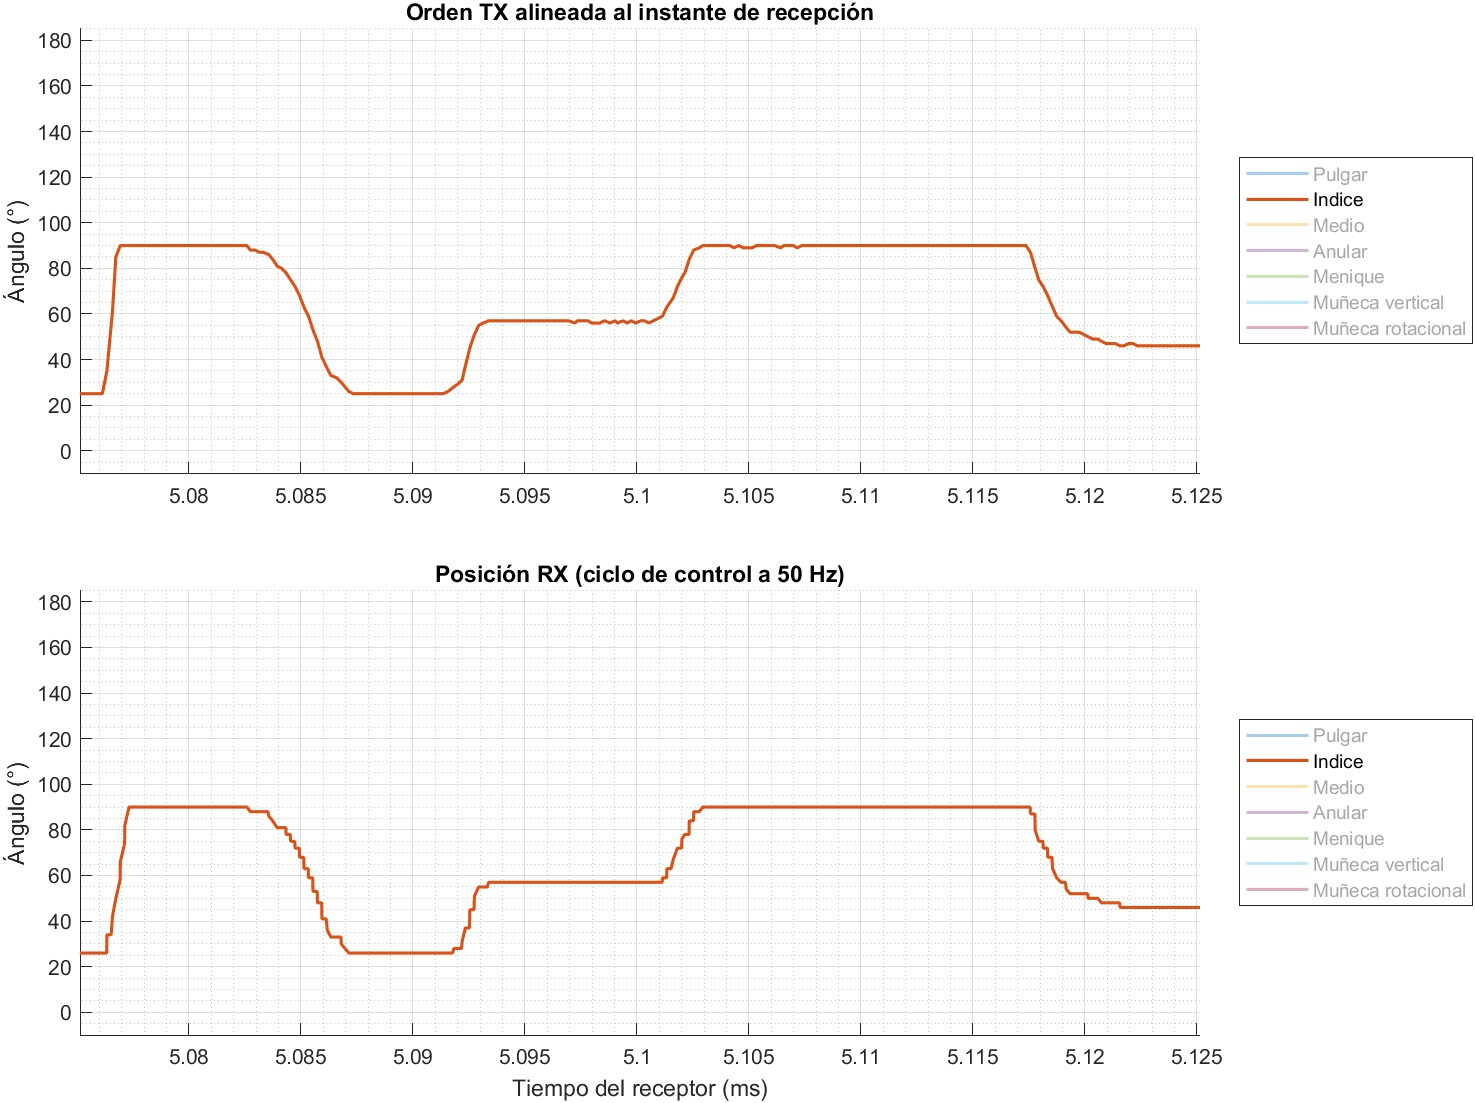
\includegraphics[width=\linewidth]{Mediciones/P16_matlab_indice.jpg}\\{\scriptsize Índice: flexiones completas y parciales}
    \column{0.5\textwidth}
    \centering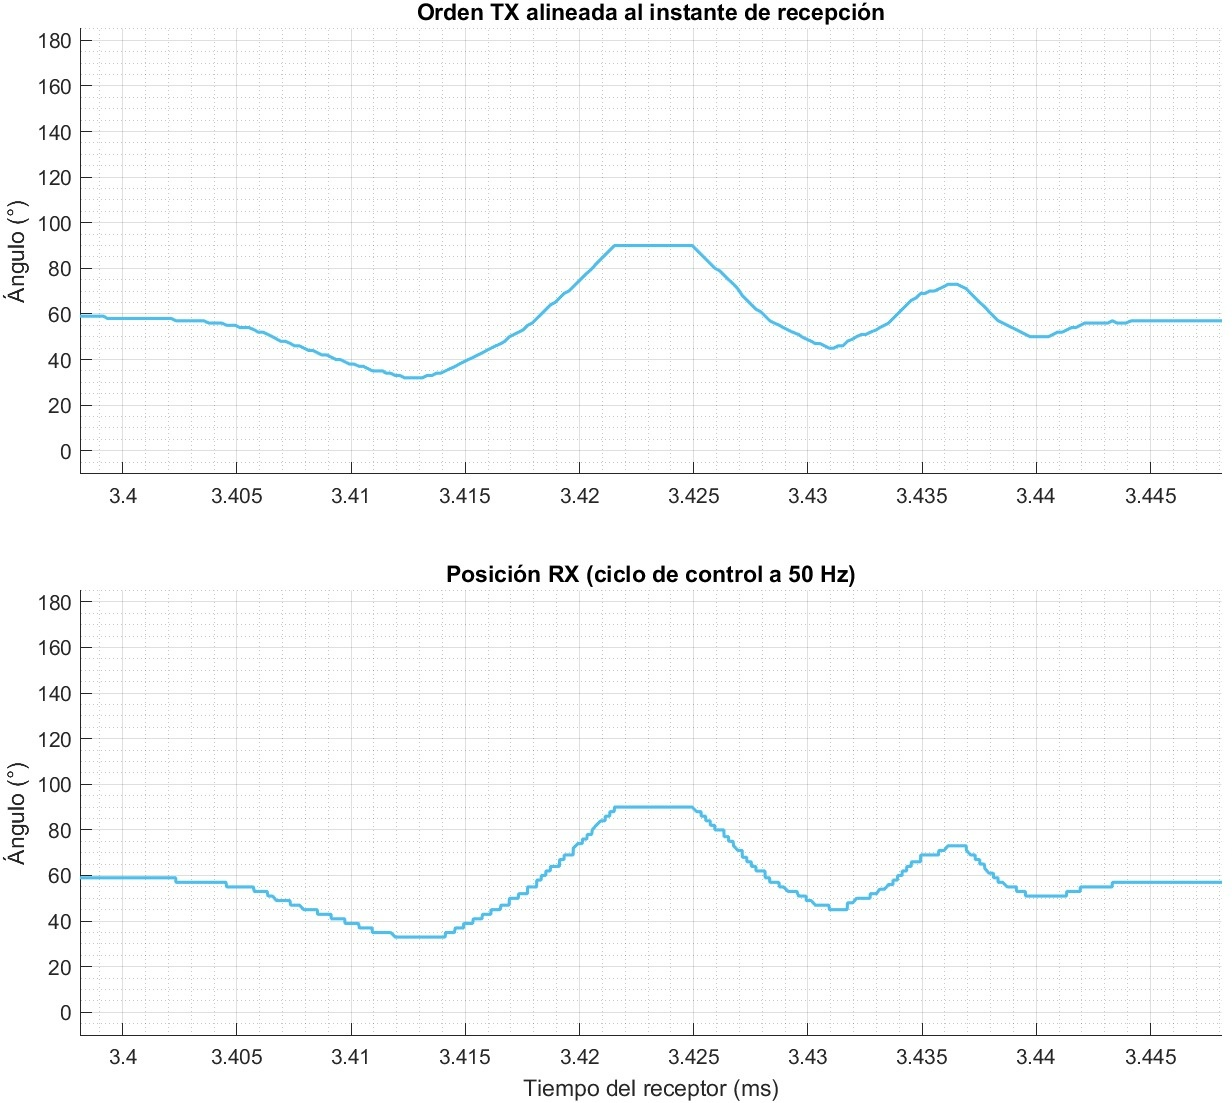
\includegraphics[width=\linewidth]{Mediciones/P16_matlab_muneca_vertical.jpg}\\{\scriptsize Muñeca vertical: saturación en \SI{90}{\degree}}
  \end{columns}
\end{frame}

\begin{frame}{Respaldo: servo bloqueado y salida de \SI{5}{\volt}}
  \begin{columns}[T]
    \column{0.5\textwidth}
    \centering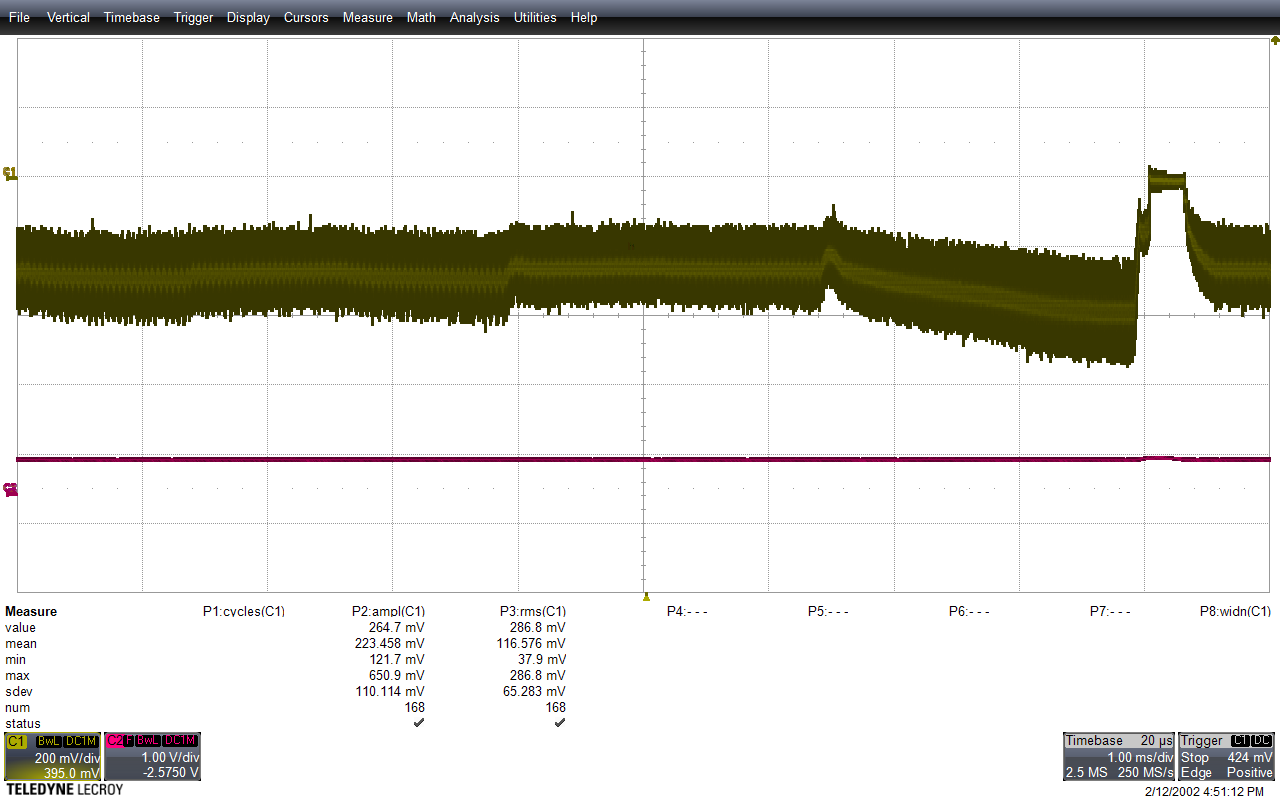
\includegraphics[width=\linewidth]{Mediciones/P03_servo_bloqueado.png}\\
    {\scriptsize Servo bloqueado a mano: \SIrange{0.55}{0.6}{\ampere} a \SI{12}{\volt}, conmutación continua.
    El corte final es el instante en que se suelta el agarre.}
    \column{0.5\textwidth}
    \centering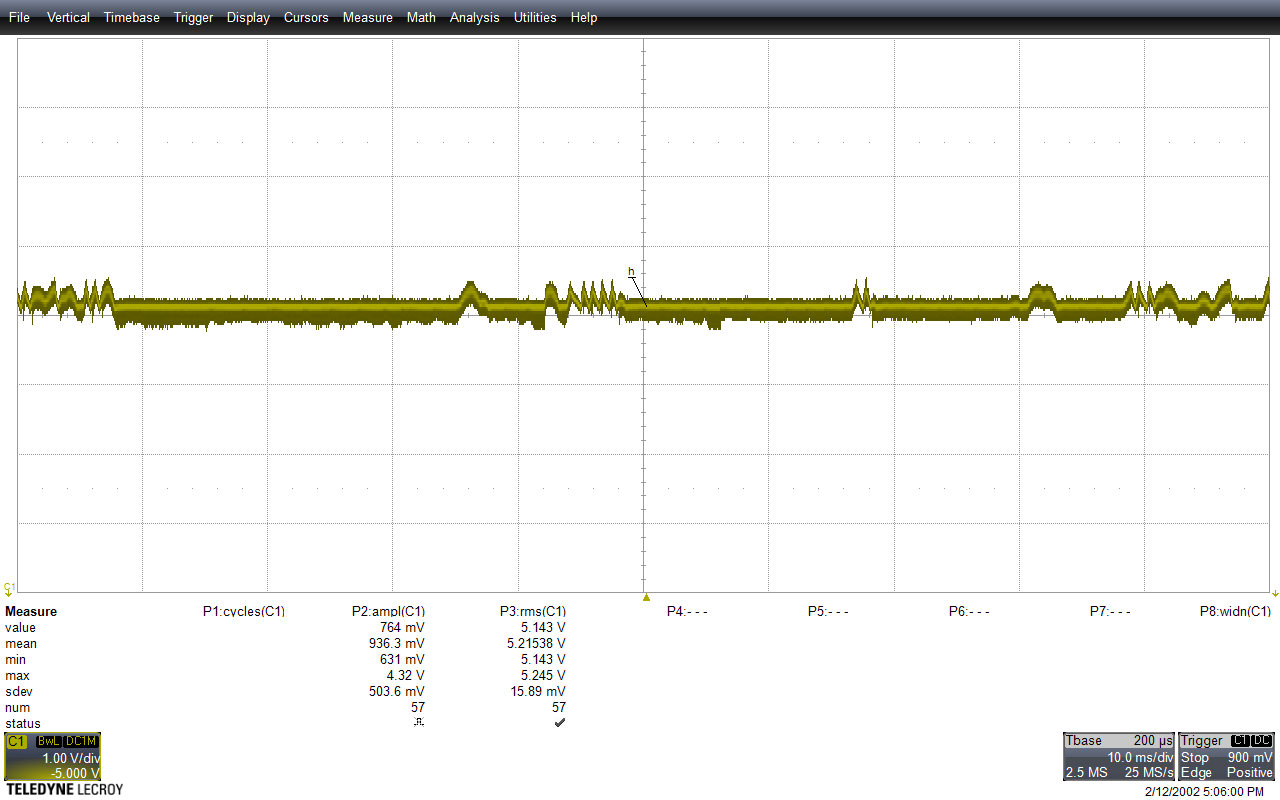
\includegraphics[width=\linewidth]{Mediciones/P02_V5_regulador.png}\\
    {\scriptsize Salida del regulador: \SIrange{5.14}{5.25}{\volt} (RMS), variación imperceptible.}
  \end{columns}
\end{frame}

\begin{frame}{Respaldo: preguntas probables}
  \small
  \begin{description}
    \item[¿Por qué ESP-NOW?] Sin router ni asociación, paquetes cortos con ACK por MAC, latencia de pocos ms; BLE tiene intervalos de conexión mayores y Wi-Fi con router agrega un salto y dependencia de infraestructura.
    \item[¿Qué pasa si se corta el enlace?] A los \SI{250}{\milli\second} la mano va a reposo en rampa; a los \SI{2}{\second} en reposo se apagan los PWM.
    \item[¿Alcanza la fuente?] Sí: peor caso medido $<\SI{0.75}{\ampere}$ a \SI{12}{\volt} frente a \SI{4}{\ampere}; por hoja de datos, 2 MG946R bloqueados suman \SI{2.4}{\ampere} y se acercan a los \SI{3}{\ampere} del regulador, por eso la rampa de velocidad.
    \item[¿Qué es el corte al final de la captura con servo bloqueado?] El instante en que se soltó el agarre del servo; no es una falla.
    \item[¿Por qué no se mide el \textit{yaw}?] El acelerómetro no lo ve y sólo con el giróscopo deriva; haría falta un magnetómetro.
    \item[¿Otro operador?] Se recalibra el guante (\texttt{c} por consola); la mano no cambia.
    \item[¿GPIO12 en el receptor?] Es pin de \textit{strapping}; no dio problemas, pero es lo primero a revisar ante una falla de arranque.
  \end{description}
\end{frame}

\end{document}
